\documentclass[webpdf,contemporary,large]{oup-authoring-template}
%% ---------------------------------------------------------------------------
%% Glaukopis: Cyber Threat Intelligence Language Model Training:
%% Optimizing Domain Specific LLM Performance
%%
%% Worth, Cardei, Alam. Formatted for the OUP contemporary
%% author-year template. Compile with pdfLaTeX.
%%
%% NOTE: This template already loads amsmath, amssymb, hyperref, graphicx,
%% url, natbib, etc. Do NOT re-load them.
%% ---------------------------------------------------------------------------

\graphicspath{{figures/}{img/}{Fig/}}

%% --- Technical-identifier macro --------------------------------------------
%% \hfid{...} renders a Hugging Face / Hugging Face-style identifier (model
%% name, dataset path, etc.) in a slightly smaller monospaced font that wraps
%% cleanly at `/`, `-`, and `_` boundaries so that long identifiers do not
%% overflow the column. Implemented via the url package (loaded by OUP class)
%% with hyphen and underscore added to the break set.
%% --------------------------------------------------------------------------
\makeatletter
\AtBeginDocument{%
  \urlstyle{tt}%
  \def\UrlBreaks{\do\/\do\-\do\_\do\.\do\:}%
}
\makeatother
\providecommand{\hfid}[1]{{\small\nolinkurl{#1}}}



%% Theorem-style declarations (OUP-standard; kept for completeness even if unused)
\theoremstyle{thmstyleone}
\newtheorem{theorem}{Theorem}
\newtheorem{proposition}[theorem]{Proposition}
\theoremstyle{thmstyletwo}
\newtheorem{example}{Example}
\newtheorem{remark}{Remark}
\theoremstyle{thmstylethree}
\newtheorem{definition}{Definition}

\begin{document}

% Venue: 38th IEEE International Conference on Tools with Artificial Intelligence (ICTAI 2026)
% See https://ictai.computer.org/2026/
% NOTE: This document still uses the OUP authoring template for layout convenience.
% Before final submission, port to the IEEE conference style (IEEEtran) and
% replace the OUP metadata macros below with the IEEEtran equivalents.
\journaltitle{IEEE ICTAI 2026}
\DOI{DOI added during production}
\copyrightyear{2026}
\pubyear{2026}
\access{Accepted at ICTAI 2026 (ictai.computer.org/2026)}
\appnotes{Conference Paper}

\firstpage{1}

\title[Glaukopis: A 32B CTI LLM via Chained IFT]{Glaukopis: Building a 32B CTI LLM Using Chained Instruction Fine-Tuning}

\author[1,3,$\ast$]{Peter J. Worth Jr.}
\author[1,3]{Ionut Cardei}
\author[2,3]{Md Tanvirul Alam}

\address[1]{\orgdiv{Department of Electrical Engineering and Computer Science}, \orgname{Florida Atlantic University}, \orgaddress{\street{777 Glades Road}, \postcode{33431}, \state{Boca Raton, FL}, \country{United States}}}

\address[2]{\orgdiv{Global Cybersecurity Institute}, \orgname{Rochester Institute of Technology}, \orgaddress{\street{1 Lomb Memorial Drive}, \postcode{14623}, \state{Rochester, NY}, \country{United States}}}

\address[3]{\orgname{Athena Security Group, LLC}, \orgaddress{\country{United States}}}

\corresp[$\ast$]{Corresponding author. \href{mailto:pworthjr@athenasecuritygrp.com}{pworthjr@athenasecuritygrp.com}}

\received{Date}{0}{Year}
\revised{Date}{0}{Year}
\accepted{Date}{0}{Year}

\abstract{Cyber threat intelligence (CTI) workflows in regulated security operations cannot in general rely on frontier proprietary models due to cost, latency, and data-handling constraints, while generic foundation models lack the schema fidelity, applied reasoning, and current-threat awareness those workflows require. This paper introduces \textbf{Glaukopis}, a methodology and working system for producing on-premises 32B-scale CTI expert language models via \textit{chained instruction fine-tuning} (chained IFT): an IFT pipeline in which the training data is materialized by typed queries against an authoritative knowledge graph---so each Alpaca-format (instruction, input, output) triple is graph-grounded rather than synthesized---and in which the supervised fine-tuning pass is decomposed into a chain of stages with distinct dataset shards and hyperparameter regimes. Glaukopis has three components: \textbf{Ariadne}, a Neo4j substrate ingesting twelve public CTI sources (ATT\&CK, ENGAGE, CAPEC, CWE, D3FEND, CVE 5.0, NVD, CISA KEV, FIRST EPSS, Sigma, ExploitDB, PoC-in-GitHub) into ${\sim}280$K nodes and ${\sim}480$K edges; \textbf{Sophia}, a graph-template generator that compiles declarative CTI reasoning patterns into IFT triples whose answers are guaranteed consistent with the graph; and a \textbf{four-stage IFT chain} (Core, +TAA, CSE, Recalibrate-32B). The v21 ship checkpoint reaches 66.3 average CTI benchmark score (vs.\ 59.0 for its Qwen-2.5-32B-Instruct base), approaching DeepSeek-V4-Pro (70.4), Gemini-3-Flash-Preview (69.8), and GPT-5.5 (72.9) at approximately two orders of magnitude lower per-evaluation cost.}

\keywords{instruction fine-tuning; chained IFT; supervised fine-tuning; small language models; cyber threat intelligence; CTI knowledge graphs; Neo4j; Ariadne; Sophia; MITRE ATT\&CK; AthenaBench; CyberSOCEval; CyberMetric}

\keywords[Abbreviations]{ATT\&CK, CAPEC, CoT, CTI, CVE, CWE, EPSS, IFT, KEV, KG, LLM, MoE, NVD, SFT, SLM, SOC, TAA, TTP, VSP}

\maketitle

\section{Introduction}

Large language models (LLMs) are now embedded throughout the cyber security workflow: they summarize threat reports, map indicators to MITRE ATT\&CK, triage vulnerabilities, draft detection rules, and answer analyst questions inside security operations centers (SOCs). Surveys of LLMs for security span vulnerability detection, malware analysis, cyber threat intelligence (CTI), phishing detection, and SOC automation, and consistently identify the same residual failure modes: hallucinations on schema-bearing fields, shallow pattern matching where causal or multi-hop reasoning is required, and a structural inability to operate on threat information more recent than the base model's pretraining cutoff \cite{levi2024cyberpal,liu2024cyberbench}.

\subsection{The operational dilemma}
\label{sec:intro-the-operational-dilemma}
The practical response in industry has been an awkward two-way split. Generic foundation models are inexpensive and easy to host but underperform on CTI-specific tasks: schema fidelity (CVE/CWE/ATT\&CK identifiers, CVSS vectors), applied reasoning (root-cause mapping, severity estimation, threat-actor attribution), and current-threat awareness are all weak. Frontier proprietary models---the largest GPT, Gemini, and DeepSeek releases---substantially close the capability gap, but their cost, latency, and data-handling characteristics are incompatible with most regulated security operations. SOCs supporting healthcare, financial services, or government workloads cannot, in general, send raw threat telemetry to a third-party API; even where the legal posture allows it, the per-evaluation cost of running a frontier model across a realistic CTI workload is prohibitive at the scale of a real analyst team.

\subsection{Chained instruction fine-tuning}
\label{sec:intro-chained-instruction-fine-tuning}
A natural alternative is to produce a small (sub-32B) language model that has been specifically post-trained on CTI material drawn from authoritative public sources, deployable on-premises behind organizational boundaries. The approach pursued in this paper, which we call \textit{chained instruction fine-tuning} (chained IFT), is a refinement of the standard IFT pipeline \cite{wei2022flan,ouyang2022instructgpt,chung2022flant5} along two axes: (i) on the \emph{data} side, every Alpaca-format (instruction, input, output) triple is materialized by a typed query against an authoritative knowledge graph rather than authored by hand or synthesized by an LLM, so each row is grounded in named graph nodes and edges traceable to public-source natural keys; and (ii) on the \emph{training} side, the supervised pass is decomposed into a chain of stages (Section~\ref{sec:intro-chained-sft}) with distinct dataset shards and hyperparameter regimes, so capabilities accumulate compositionally and per-axis regressions are attributable to specific stages. Both axes are refinements of, not departures from, IFT as established by FLAN, InstructGPT, and FLAN-T5. The closest neighbors in the literature are IBM's CyberPal.AI and the SecKnowledge follow-on, which couple expert-curated instruction schemas with chain-of-thought enrichment \cite{levi2024cyberpal,levi2025toward}, and the SEvenLLM and CyberBench efforts, which adapt smaller open models to security through hand-crafted or LLM-synthesized instruction corpora \cite{ji2024sevenllm,liu2024cyberbench}. Section~\ref{sec:ift-structured} situates chained IFT within these neighbors and within the wider graph-grounded-IFT line.

\subsection{The Glaukopis system}
\label{sec:intro-the-glaukopis-system}
\textbf{Glaukopis} is the working instantiation of chained IFT described in this paper. It has three named components, each developed in detail in a later section:

\begin{itemize}
  \item \textbf{Ariadne} (Section~\ref{sec:cti-kg}), a Neo4j knowledge-graph substrate that ingests twelve public CTI sources spanning offensive technique catalogues (ATT\&CK, ENGAGE), weakness and attack-pattern taxonomies (CWE, CAPEC), defensive countermeasures (D3FEND), vulnerability records (CVE 5.0, NVD), exploitation signals (CISA KEV, FIRST EPSS), detection content (Sigma), and weaponized-exploit evidence (ExploitDB, PoC-in-GitHub) into approximately $280{,}000$ nodes and $480{,}000$ edges, refreshed daily for current-threat coverage.

  \item \textbf{Sophia} (Section~\ref{sec:ariadne-templates}), a graph-template generator that compiles declarative CTI reasoning patterns into Alpaca-format instruction triples whose outputs are computed directly from Cypher queries against Ariadne. Sophia supports positive and negative examples, cross-schema reasoning chains (e.g., CVE$\to$CWE$\to$CAPEC$\to$ATT\&CK), and incremental regeneration aligned to specific time windows---a property that lets the training corpus track the threat landscape as it evolves.

  \item \textbf{A four-stage IFT chain} (Section~\ref{sec:glaukopis-sft}) that turns Sophia-generated triples into a sequence of cumulative checkpoints---Core, +TAA, CSE, and Recalibrate-32B---each with its own dataset shard, hyperparameter regime, and intended capability outcome. Chaining the stages, rather than mixing all training data into one pass, is what makes per-axis ablation, incremental refresh, and known-trade-off recovery tractable in this pipeline. The principle is reviewed in Section~\ref{sec:intro-chained-sft}.
\end{itemize}

\subsection{Headline result}
\label{sec:intro-headline-result}
The ship checkpoint produced by the v21 vintage of this pipeline, \hfid{asg-ai/athena-cti-sft-qwen25-32b-v21-recal-32b}, reaches an average CTI-benchmark score of 66.3 across AthenaBench, CyberSOCEval, and CyberMetric. The same architecture's base instruct model (\hfid{Qwen/Qwen2.5-32B-Instruct}) scores 59.0 on the same suite---so the chained-IFT recipe adds 7.3 points without changing the parameter count or runtime footprint. On the CTI-only averages reported in this paper, the ship checkpoint \textbf{exceeds Google's Gemini-2.5-Flash} (66.3 vs.\ 63.4 on Avg CTI Benchmark and 62.9 vs.\ 57.9 on Avg CTI Test) and runs \textbf{essentially even with DeepSeek-V3.2-Exp} (66.3 vs.\ 66.0 on Avg CTI Benchmark; 62.9 vs.\ 62.2 on Avg CTI Test; DeepSeek slightly ahead on the with-MMLU composite). It then sits within 4--7 points of the leading frontier reference points---DeepSeek-V4-Pro (70.4), Gemini-3-Flash-Preview (69.8), and GPT-5.5 (72.9)---at approximately two orders of magnitude lower per-evaluation cost. Detailed numbers are reported in Section~\ref{sec:results}.

\subsection{Main contributions}
\label{sec:intro-main-contributions}
The principal contributions of this paper are as follows:

\begin{enumerate}
  \item We introduce \textbf{chained instruction fine-tuning} (chained IFT) as a refinement of the standard IFT pipeline along two axes---graph-grounded data construction and multi-stage SFT scheduling---and locate it within the FLAN/InstructGPT/FLAN-T5 lineage and the CyberPal.AI / SecKnowledge cyber-security IFT line (Section~\ref{sec:ift-slm}).

  \item We describe \textbf{Ariadne} (Section~\ref{sec:cti-kg}), a Neo4j CTI knowledge-graph substrate that ingests twelve public CTI sources into approximately $280{,}000$ nodes and $480{,}000$ edges with explicit, documented refresh discipline, and \textbf{Sophia} (Section~\ref{sec:ariadne-templates}), a graph-template generator that compiles declarative CTI reasoning patterns into Alpaca-format instruction triples computed by typed Cypher queries against Ariadne. Together they form a complete, auditable training-data pipeline in which every row maps to specific public-source identifiers.

  \item We specify and ship a \textbf{four-stage chained-IFT recipe} (Section~\ref{sec:glaukopis-sft})---Core, +TAA, CSE, and Recalibrate-32B---with full per-stage hyperparameters and dataset shards, and report the v21 strict-reproducibility experiment that isolated data-build non-determinism in the template-generation substrate from recipe-level drift (Section~\ref{sec:glaukopis-v21-templates}).

  \item We report a \textbf{benchmark evaluation portfolio} spanning AthenaBench, CyberSOCEval, CyberMetric (2K and 10K), and MMLU-Pro as a decoupled general-intelligence reference, with three explicit averaging schemes whose differences are themselves diagnostic (Section~\ref{sec:results-averaging}); a \textbf{cost analysis} that places accuracy alongside per-evaluation dollar cost as a first-class metric (Section~\ref{sec:results-cost}); and an \textbf{explicit data-contamination protocol} that distinguishes verbatim from structural overlap between training and evaluation data, with auditable per-shard enforcement (Appendix~\ref{app:contamination}).

  \item We \textbf{release the source code and configuration} for Ariadne, Sophia, the chained-IFT training scripts, and the evaluation harness as an open-source repository at \url{https://github.com/Athena-Software-Group/Glaukopis} \cite{glaukopis2026repo}, together with the cumulative Hugging Face checkpoints for the Qwen-2.5-32B-Instruct ship and the cross-architecture ports.
\end{enumerate}

\subsection{Paper structure}
\label{sec:intro-paper-structure}
The remainder of the paper is organized as follows:
\begin{itemize}
  \item Section~\ref{sec:ift-slm} reviews instruction fine-tuning, its chained refinement, the graph-grounded IFT line in cyber security, and the small-language-model literature that motivates the Glaukopis approach.
  \item Section~\ref{sec:benchmarks} surveys cyber security LLM benchmarks and develops the four-suite evaluation portfolio (AthenaBench, CyberSOCEval, CyberMetric, MMLU-Pro) used in this paper.
  \item Section~\ref{sec:cti-kg} introduces Ariadne---the Athena CTI knowledge-graph substrate---and Sophia, the graph-template generator that compiles CTI reasoning patterns into instruction triples consumed by the Glaukopis training pipeline.
  \item Section~\ref{sec:glaukopis} describes Glaukopis itself: the v21 template-generation vintage, the four-stage IFT chain, and the evaluation harness.
  \item Section~\ref{sec:results} presents the v21 evaluation results across the benchmark portfolio.
  \item Section~\ref{sec:open-challenges} closes with open challenges and research directions.
\end{itemize}

\section{Instruction Fine-Tuning: Foundations and Cyber Security Practice}
\label{sec:ift-slm}

This section summarizes the IFT background that Glaukopis builds on. We touch each topic only to the depth needed to situate the design choices that follow: the foundational IFT papers (\S\ref{sec:ift-foundations}); the multi-stage refinement we call \emph{chained IFT} (\S\ref{sec:intro-chained-sft}); the graph-grounded IFT lineage in which the Sophia generator sits (\S\ref{sec:ift-structured}); the cyber-security--specific IFT line led by IBM's CyberPal.AI work (\S\ref{sec:ift-cyber}); and the small-language-model literature that motivates the on-premises 32B deployment target (\S\ref{sec:ift-slm-cyber}).

\subsection{IFT Foundations: FLAN, InstructGPT, FLAN-T5}
\label{sec:ift-foundations}

Pretrained LLMs are optimized for next-token prediction on broad text corpora, not for following user instructions. Instruction fine-tuning (IFT) fine-tunes such models on labeled (instruction, optional context, target output) datasets, maximizing log-likelihood of the reference output given the instruction and context \cite{wei2022flan,ouyang2022instructgpt}. As a category, IFT is one instantiation of supervised fine-tuning (SFT); we use ``IFT'' throughout this paper as the dominant convention in the cyber security literature on the same family of methods. The modern formulation rests on three foundational papers from 2021--2022.

\textbf{FLAN} \cite{wei2022flan} demonstrated that fine-tuning a pretrained LLM on a diverse mix of NLP tasks expressed uniformly as natural-language instructions yields strong zero-shot generalization to unseen tasks. The central insight---that instruction-following is a \emph{learnable} capability rather than an emergent property of scale alone---established IFT as a distinct training paradigm and motivates the use of instruction-formatted training rows in every IFT pipeline since, Glaukopis included.

\textbf{InstructGPT} \cite{ouyang2022instructgpt} introduced the three-phase pipeline that remains the basis for many production LLMs: (i) supervised instruction fine-tuning on human-written instruction--response pairs, (ii) preference modeling, and (iii) reinforcement learning from human feedback (RLHF). Its key finding---that relatively small instruction-tuned models can be preferred over much larger unaligned ones---is the load-bearing argument for the small-model strategy this paper pursues. The order-of-stages matters: each phase has its own data and objective, and the staged structure is itself part of what makes the final behavior controllable. The chained-IFT recipe in Section~\ref{sec:glaukopis-sft} is a CTI-specialized version of the same principle on the SFT side.

\textbf{FLAN-T5} \cite{chung2022flant5} scaled the instruction corpus to thousands of tasks and showed that IFT consistently improves downstream performance across model sizes, that the gains persist as base models scale, and that the diversity and structure of the instruction data matter at least as much as parameter count. This is the empirical license for the Glaukopis design choice to invest heavily in instruction-data structure (via Sophia and Ariadne) at a fixed 32B parameter budget rather than chasing more parameters at fixed data quality.

These three results---learnable instruction-following, staged training as a control interface, and structured-data primacy---are the foundations Glaukopis stands on directly. Two further refinements specific to the present work are reviewed next.

\subsection{Chained IFT: Multi-Stage Supervised Fine-Tuning}
\label{sec:intro-chained-sft}

A recurring design choice in modern post-training is to compose several IFT stages into a chain rather than to perform a single, monolithic instruction tune. In a chained IFT pipeline, the base pretrained model is adapted to its target deployment through an ordered sequence of stages, each with its own dataset shard, optimization hyperparameters, and intended outcome; the output checkpoint of each stage becomes the initialization for the next. Capabilities accumulate compositionally rather than competing for capacity within a single fine-tune, and individual stages can be re-run when their underlying data changes, attributing observed gains or regressions to specific stages. Figure~\ref{fig:glaukopis-chained-ift} illustrates the overall shape: graph-grounded IFT shards from Sophia feed an ordered four-stage chain in which each stage has its own training objective and hyperparameter regime, and the benchmark suite serves as the measurement criterion at every cumulative checkpoint.

\begin{figure*}[t]
\centering
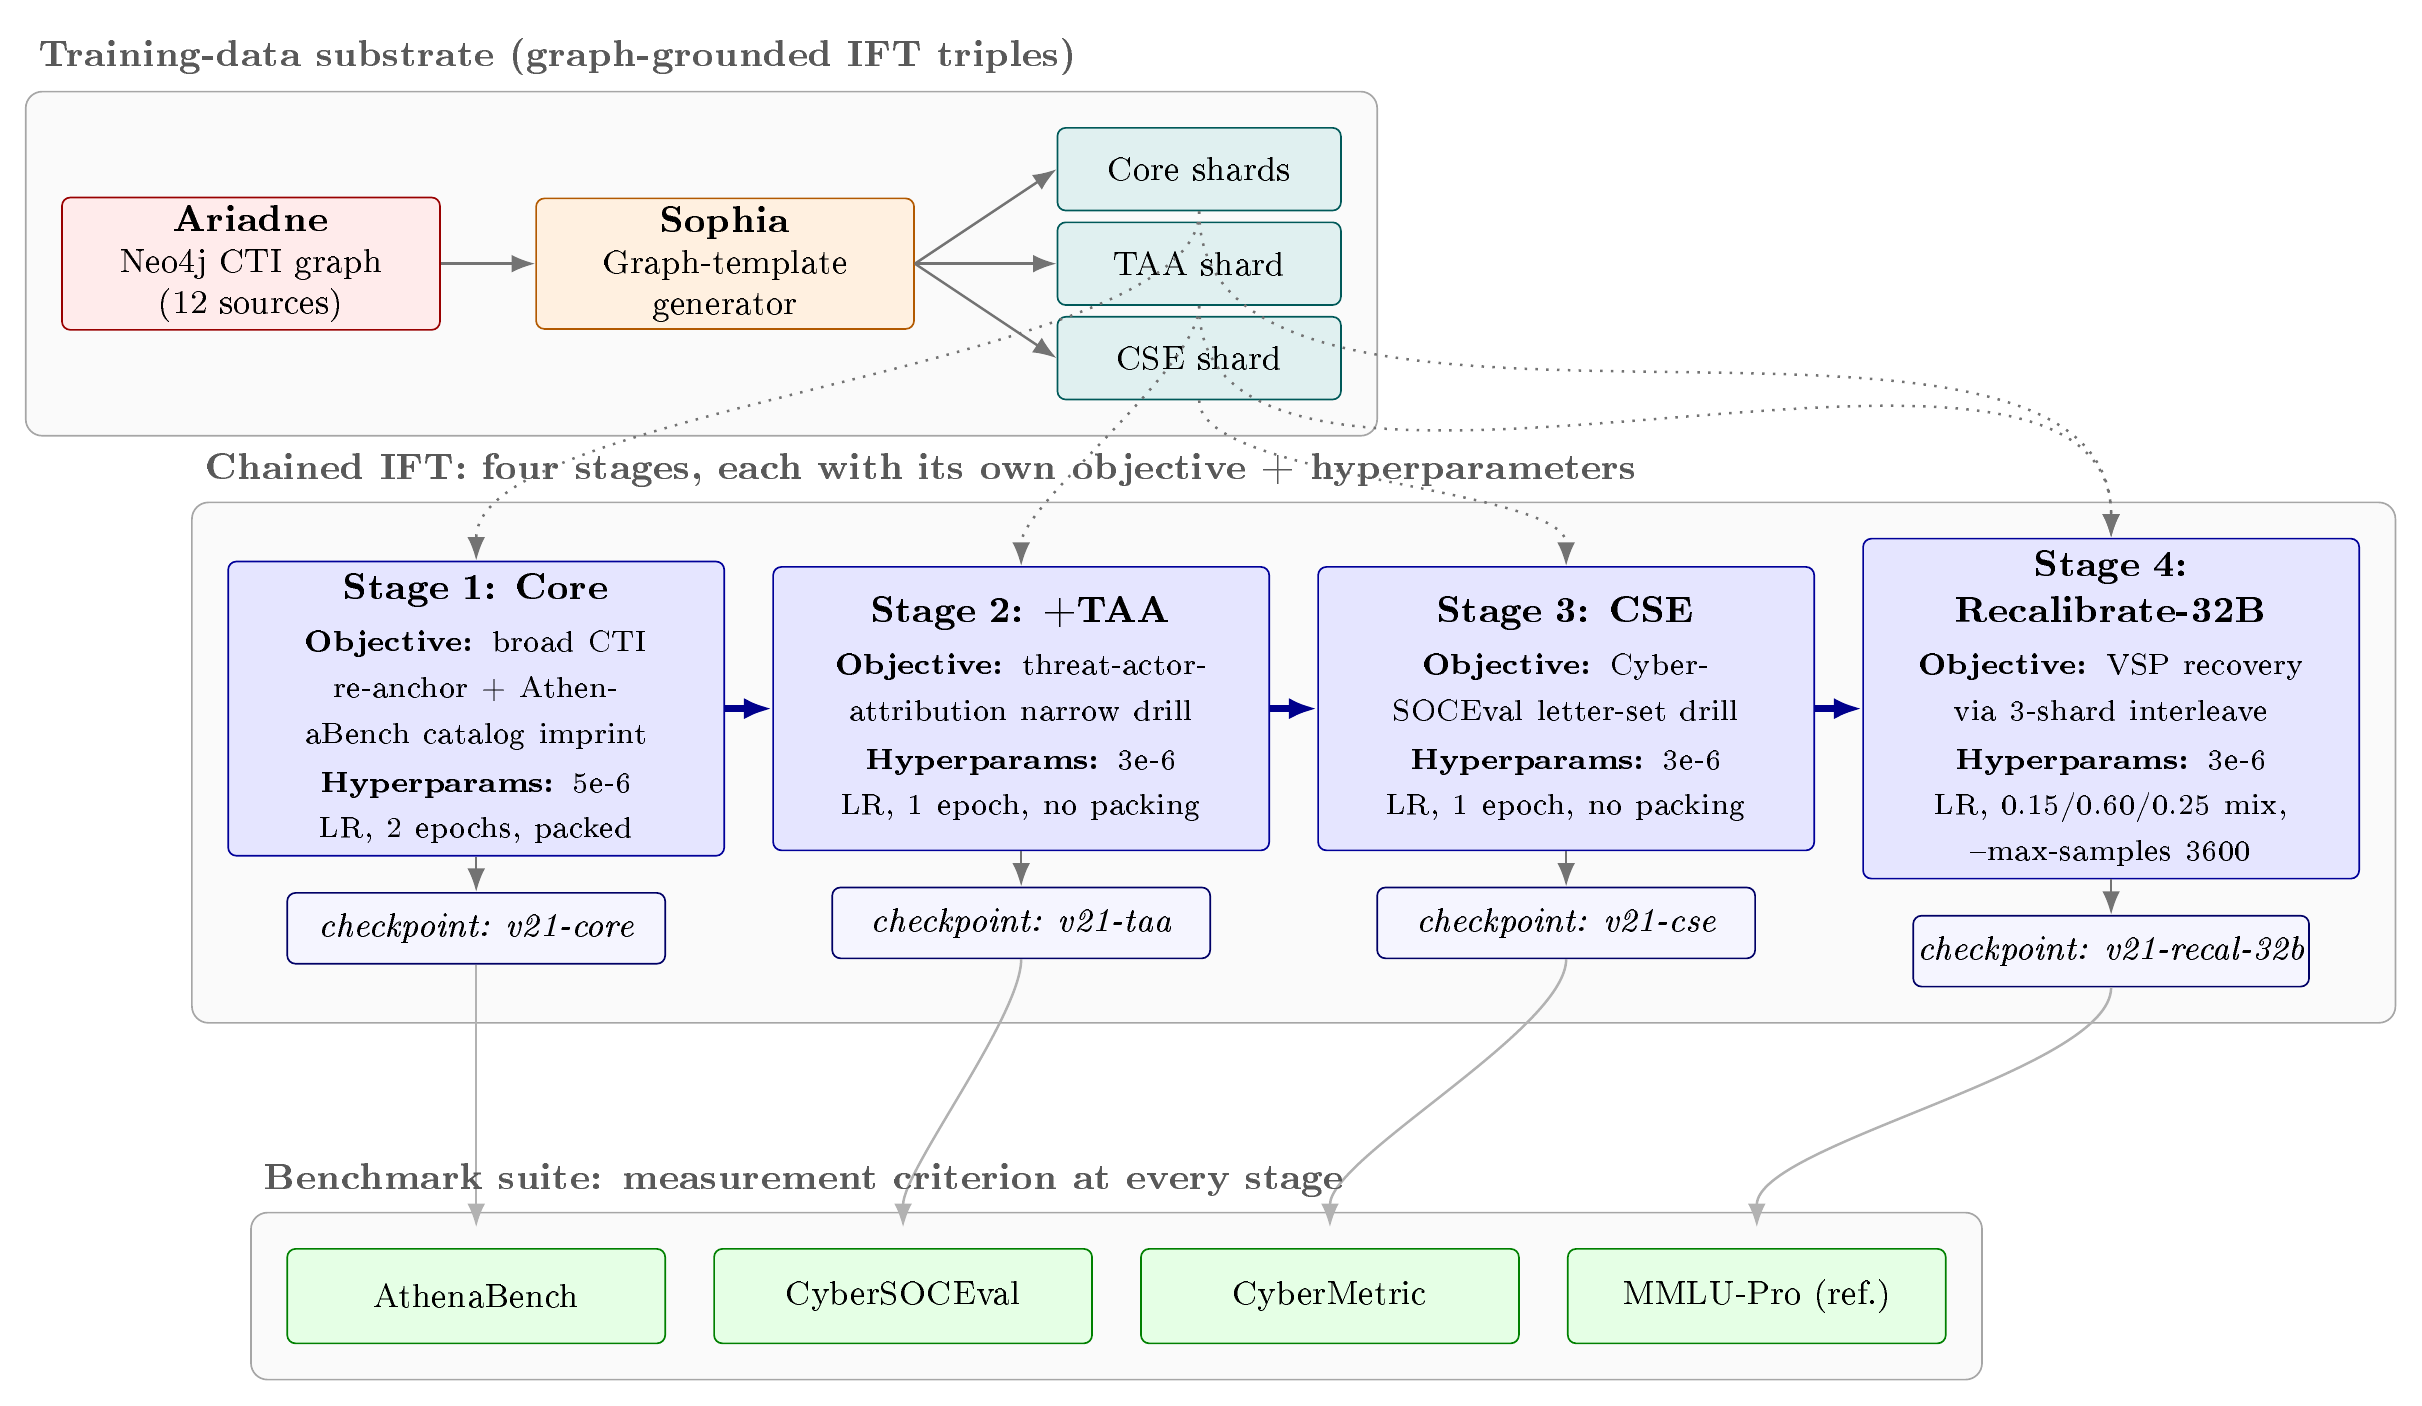
\includegraphics[width=\textwidth]{figures/glaukopis_chained_ift.png}
\caption[]{\textbf{The chained-IFT pattern.} Sophia compiles typed graph queries against Ariadne into Alpaca-format IFT triples, sharded into Core, TAA, and CSE manifests. The four-stage IFT chain consumes these shards in order: each stage has its own \emph{objective} (broad CTI re-anchor for Core, narrow drills for TAA and CSE, recalibration for Stage~4) and its own \emph{hyperparameters} (learning rate, epoch count, packing, and---in Stage~4---an explicit three-shard interleave). Each stage pushes a cumulative checkpoint (\hfid{v21-core}, \hfid{v21-taa}, \hfid{v21-cse}, \hfid{v21-recal-32b}), each of which can be evaluated independently against the AthenaBench / CyberSOCEval / CyberMetric / MMLU-Pro benchmark suite. The benchmark suite is the measurement criterion at every stage, supporting per-stage ablation in addition to producing a single ship checkpoint.}
\label{fig:glaukopis-chained-ift}
\end{figure*}

The motivations for this pattern recur across the literature. Separating broad domain absorption from precise task behavior reduces destructive interference; training jointly on noisy domain text and structured task triples tends to either underfit the structured task or overfit narrow templates, while staging gives each objective its own learning-rate, schedule, and packing regime \cite{gururangan2020dontstop,ouyang2022instructgpt}. Reasoning supervision is more effective when layered on top of a model that already commands the underlying domain vocabulary and task formats than when it is mixed in from the start; this motivated the chain-of-thought enrichment stages in CyberPal/SecKnowledge~2.0 \cite{wei2022cot,levi2025toward}. And staging makes pipelines incrementally refreshable, which matters in a domain (CTI) where source data turns over weekly.

Glaukopis (Section~\ref{sec:glaukopis}) adopts this pattern with a four-stage chain---Core, +TAA, CSE, and Recalibrate-32B---tailored to graph-template-generated CTI instruction data and the AthenaBench / CyberSOCEval / CyberMetric evaluation portfolio. The CyberPal.AI / SecKnowledge line operationalizes a closely related staging discipline on a different data construction pipeline \cite{levi2024cyberpal,levi2025toward}.

\subsection{Graph-Grounded IFT: Three Converging Traditions}
\label{sec:ift-structured}

The second refinement Glaukopis adopts is on the data-construction side: every IFT triple is materialized by a typed query against an authoritative knowledge graph (Ariadne) rather than authored by hand or synthesized by an LLM. This is not itself a new paradigm but a discipline that has emerged from the convergence of three research lines.

\textbf{Schema- and grammar-constrained generation.} The semantic parsing and constrained-decoding literature established the precedent that target outputs can be required to conform to a formal grammar or schema (logical forms, SQL queries, knowledge-base triples), and that pairs of natural-language inputs and structured outputs can be \emph{computed} by sampling the grammar or executing queries against a reference database rather than authored manually. This is the conceptual origin of ``every training row should be computable, not authored.''

\textbf{Knowledge-graph-grounded QA and KG-to-text.} A second line contributes the specific pattern of materializing training rows by graph traversal: a typed query against a knowledge graph returns a subgraph that is rendered, by template or learned model, into a natural-language question--answer pair. The CTI-specific instantiations reviewed in Section~\ref{sec:cti-kg-llms} (Fieblinger et al.\ \cite{fieblinger2024kg}, Open-CyKG \cite{wu2022opencykg}, CTIKG \cite{yu2024ctikg}, K-CTIAA \cite{zhao2024kctiaa}, CyberKG \cite{zhang2023cyberkg}) demonstrate that LLMs can be trained against graph-derived QA corpora with measurable benefits when the underlying graph is the authoritative source of truth.

\textbf{Expert-schema-driven IFT for cyber security.} The third line---IBM's CyberPal.AI \cite{levi2024cyberpal} and SecKnowledge~2.0 \cite{levi2025toward}---demonstrates that an instruction corpus structured by expert-authored schemas can transform a general SLM into a cyber security expert at the 4--20B scale. CyberPal does not require the answers themselves to be materialized from a knowledge graph, but the discipline of constraining the instruction shape via expert schemas is conceptually adjacent.

Glaukopis combines all three: the Ariadne graph schema (Tradition 1) defines the typed CTI substrate; every Sophia-generated training row is materialized by a Cypher query against the populated graph (Tradition 2); and the templates that drive those queries are CTI-specific reasoning patterns authored or curated by domain experts (Tradition 3), with chained IFT (\S\ref{sec:intro-chained-sft}) as the orthogonal training-side complement.

\subsection{Instruction Fine-Tuning for Cyber Security}
\label{sec:ift-cyber}

Cyber security imposes specific demands on IFT: technical jargon and heterogeneous schemas (CVE, CWE, CAPEC, ATT\&CK); a requirement for structured, evidence-grounded outputs (CVSS vectors, CWE IDs, ATT\&CK mappings); and rapid concept drift as new vulnerabilities and campaigns appear. Several efforts address these via cyber-specific instruction data. \textbf{SEvenLLM} \cite{ji2024sevenllm} constructs a bilingual cyber security instruction dataset and the SEvenLLM-Bench benchmark from real incident reports, converting raw text into QA, extraction, and reasoning tasks. \textbf{CyberBench / CyberInstruct} \cite{liu2024cyberbench} provide cyber-specific instruction tasks drawn from logs, alerts, and vulnerability descriptions, with the CyberBench evaluation suite for the resulting models. \textbf{Lily-Cybersecurity-7B} \cite{liu2024cyberbench} is a Mistral-7B fine-tune on hand-crafted hacking and security instructions, later LLM-enriched for style.

The closest neighbor to Glaukopis in this family is the IBM \textbf{CyberPal.AI} line. The original CyberPal release \cite{levi2024cyberpal} built SecKnowledge by mining MITRE ATT\&CK, Sigma rules, SIEM rules, adversary emulation plans, and threat reports, and then using domain experts to define instruction schemas (e.g., mapping logs to ATT\&CK techniques, suggesting mitigations) and populate them semi-automatically. The follow-on \emph{Toward Cybersecurity-Expert Small Language Models} \cite{levi2025toward} extended this to SecKnowledge~2.0 with chain-of-thought rationale enrichment and an expert-in-the-loop validation pipeline, training cyber security expert SLMs at 4--20B parameters that rival much larger general models on CTI tasks.

CyberPal demonstrates that expert-curated, knowledge-grounded instruction data can transform general LLMs into specialized CTI assistants with strong reasoning and reduced hallucination. Glaukopis sits in the same family with three differences worth noting up front: (i) every training row is materialized from the Ariadne CTI graph rather than synthesized from mixed structured/unstructured sources; (ii) the SFT pass is decomposed into a four-stage chain with explicit per-axis recovery (Section~\ref{sec:glaukopis-sft}); and (iii) the target is the 32B parameter scale, which we find is the most efficient point for CTI on the dense architectures we tested (Section~\ref{sec:results}).

\subsection{Small Language Models for Cyber Security}
\label{sec:ift-slm-cyber}

Small language models---roughly 2--20B parameters, with 32B at the natural upper bound for on-premises deployment---are increasingly attractive for cyber security. The deployment constraints are concrete: SOC and CTI environments often require on-premises, air-gapped, or bring-your-own-model setups for regulatory and confidentiality reasons; incident response and detection engineering need low-latency, high-volume inference; and well-targeted SLMs can be retrained as CTI sources evolve more cheaply than frontier-scale models. CyberPal~2.0 \cite{levi2025toward} pursued this explicitly at the 4--20B range and showed that well-instruction-tuned SLMs can match or exceed larger general models on CTI tasks, especially when CoT-enriched.

The Glaukopis target sits one tier above this band at 32B parameters. The choice is driven by the Section~\ref{sec:results} finding that general-knowledge erosion (Section~\ref{sec:results-headline}) under any aggressive CTI IFT recipe is parameter-count-graded: 8B ports lose 17.6--20.6 MMLU-Pro points to specialization, 14B loses 13.9, 32B loses 11.6. 32B is therefore the smallest deployment-feasible scale at which the trade-off curve is acceptable for our target workloads; results below 32B are reported as cross-architecture ports rather than as the headline ship. The emerging pattern is that \emph{graph-grounded IFT + chaining + a 32B base} is a pragmatic recipe for CTI: linguistic knowledge from pretraining, domain semantics and task formats from graph-materialized IFT, capability accumulation from chaining, deployability from the parameter budget. The Glaukopis instantiation of this recipe is described in Section~\ref{sec:glaukopis}.


\section{Cyber Security LLM Benchmarks}
\label{sec:benchmarks}

\subsection{Why Cyber-Security-Specific Benchmarks?}

General benchmarks such as GLUE, MMLU, and BIG-Bench measure broad language understanding and world knowledge, and certain security-adjacent capabilities (e.g., information-security multiple-choice questions in MMLU) appear as minor subsets, but these suites are not designed to probe the workflows that actually define security practice. They lack the structured schemas, evidence-grounded reasoning, and threat-current content that distinguish cyber security tasks from general knowledge work. The gaps that motivate domain-specific benchmarking are concrete:

\begin{itemize}
  \item \textbf{Schema fidelity.} Security workflows operate over standardized identifiers and structured artifacts (CVE, CWE, CAPEC, CVSS vectors, MITRE ATT\&CK technique IDs, STIX/TAXII objects). General benchmarks do not test whether a model produces well-formed outputs in these schemas, which is the difference between a usable assistant and one that requires constant human re-formatting.
  \item \textbf{Applied reasoning.} CTI and SOC analysts rarely need pure recall; they need chained inferences (e.g., from a CVE description to the underlying weakness class, then to relevant attack patterns and detection opportunities), severity estimation under partial information, and abductive attribution from observed TTPs. These reasoning shapes are largely absent from general benchmarks.
  \item \textbf{Temporal relevance.} The threat landscape evolves on a weekly cadence (new CVEs, new APT activity, new exploitation campaigns), so static benchmarks rapidly drift from operational reality and become measures of stale memorization rather than current competence \cite{alam2025athenabench}.
  \item \textbf{Data contamination.} Many cyber security sources (MITRE ATT\&CK, the NVD, public threat reports) are heavily represented in LLM pretraining corpora. A static benchmark drawn from those same sources risks measuring recall of training data rather than genuine reasoning, an effect that dynamic benchmarks aim to mitigate \cite{alam2025athenabench}.
\end{itemize}

In response, the past two years have seen a rapid expansion of cyber-security-specific benchmarks, which can be grouped roughly into four overlapping families: \emph{knowledge benchmarks}, focused on factual recall of security concepts and terminology; \emph{secure-coding and offensive-capability benchmarks}, focused on whether models help or hinder secure software development and adversarial use; \emph{CTI and SOC benchmarks}, focused on applied threat-intelligence and operations reasoning; and \emph{dynamic / live-source benchmarks}, focused on resistance to data staleness and contamination. Important entries include:

\begin{itemize}
  \item \textbf{CyberMetric.} A retrieval-augmented, certification-style multiple-choice benchmark by Tihanyi et al.\ covering nine cyber security domains, released in graduated sizes (80, 500, 2000, and 10\,000 questions) to support both rapid evaluation and statistically robust comparison \cite{tihanyi2024cybermetric}.
  \item \textbf{SecEval.} A multiple-choice benchmark of cyber security knowledge questions spanning multiple security subdomains, used to evaluate factual coverage of foundation models on standard certification-style content \cite{hu2024seceval}.
  \item \textbf{CyberBench.} A multi-task benchmark for cyber security LLMs that includes classification, question answering, and log/report analysis, accompanied by the CyberInstruct training corpus used by the same authors to build cyber-tuned models \cite{liu2024cyberbench}.
  \item \textbf{CTIBench.} A dedicated CTI benchmark covering CTI knowledge, root-cause mapping, vulnerability severity prediction, threat-actor attribution, threat-knowledge graph construction, and attack-technique extraction; constructed from curated CTI corpora and designed for reasoning-intensive evaluation \cite{alam2024ctibench}.
  \item \textbf{SEvenLLM-Bench.} A bilingual CTI benchmark derived from real incident reports, designed alongside the SEvenLLM-Instruct dataset and emphasizing cross-lingual security comprehension \cite{ji2024sevenllm}.
  \item \textbf{Purple Llama CyberSecEval and CyberSecEval~2.} Benchmarks from Meta evaluating secure-code generation, susceptibility to assisting with cyberattacks, prompt-injection robustness, and related risk dimensions \cite{bhatt2023purplellama,bhatt2024cyberseceval2}.
  \item \textbf{WMDP.} The Weapons of Mass Destruction Proxy benchmark by Li et al.\ includes a cyber security subset measuring potentially hazardous cyber-offense knowledge and is widely used to study unlearning and safety-capability tradeoffs in security-adjacent capabilities \cite{li2024wmdp}.
  \item \textbf{AthenaBench.} A dynamic CTI benchmark that draws from live sources (MITRE ATT\&CK, NVD, CISA advisories, threat reports) and explicitly targets the staleness and contamination problems that limit static suites; discussed in detail below \cite{alam2025athenabench}.
\end{itemize}

Together, these benchmarks shift evaluation from generic question answering toward security-aware reasoning, but they cover very different surfaces---factual recall, secure-code generation, applied CTI reasoning, and dynamic resistance to drift---and no single benchmark is sufficient on its own. Glaukopis is therefore evaluated against a portfolio of complementary suites, with particular weight on AthenaBench (which directly targets dynamic CTI reasoning), CyberMetric at the 2\,000- and 10\,000-question tiers (which provides statistically robust factual coverage), and CyberSOCEval's malware and threat-intelligence test suites (which probe operationally relevant SOC reasoning).\footnote{Detailed descriptions of the three suites used in this paper's evaluation portfolio---CyberMetric, CyberSOCEval, and AthenaBench---are provided in Appendix~\ref{app:benchmarks}.}

\subsection{Relationship to the Athena Training Pipeline}

AthenaBench and Glaukopis (powered by the Sophia graph-template generator over the Ariadne CTI substrate, both detailed in Section~\ref{sec:cti-kg}) are complementary components of a full CTI LLM lifecycle:

\begin{itemize}
  \item \textbf{Training side (Sophia / Ariadne).} Sophia compiles CTI reasoning patterns into Cypher queries over the Ariadne graph (ATT\&CK, CVE, CAPEC, CWE, ENGAGE, D3FEND, etc.) and emits instruction triples that drill CTI knowledge, multi-hop reasoning, negative cases, and structured outputs \cite{cardei2025ift}.
  \item \textbf{Evaluation side (AthenaBench).} Dynamically constructs CTI tasks from the same or similar underlying sources (ATT\&CK, NVD, CISA, threat reports) but with different pipelines and sampling strategies, providing independent, evolving test sets to evaluate model generalization \cite{alam2025athenabench}.
\end{itemize}

Many of Sophia's template patterns directly mirror AthenaBench tasks:
\begin{itemize}
  \item CVE$\rightarrow$CWE reasoning templates align with RCM.
  \item Templates that traverse CVE$\rightarrow$CWE$\rightarrow$CAPEC$\rightarrow$ATT\&CK map onto knowledge and mitigation reasoning tested in CKT and RMS.
  \item Templates involving malware, techniques, platforms, and data components parallel the kind of ``who uses what and how is it detected'' reasoning central to CTI analysis and attack technique extraction tasks \cite{cardei2025ift}.
\end{itemize}

Sophia's incremental generation features (version and timestamp filtering) make it possible to align the training data's recency with AthenaBench's dynamic evaluation horizon, mitigating data leakage while ensuring models are trained on approximately the same vintage of CTI as they are evaluated on \cite{cardei2025ift,alam2025athenabench}.

This alignment positions the Sophia + Ariadne pipeline as a natural training counterpart to AthenaBench's evaluation side, much as SecKnowledge and CyberPal models are paired with CTI benchmarks in IBM's work \cite{levi2024cyberpal,levi2025toward}. The next section describes the data substrate that makes this alignment concrete: Ariadne, the populated Neo4j CTI graph from which every Glaukopis training row is materialized.

\section{Ariadne: A Knowledge Graph for CTI SFT}
\label{sec:cti-kg}

\subsection{CTI Concepts and Workflows}

Cyber Threat Intelligence (CTI) is commonly defined as the collection, analysis, and dissemination of information about threats and adversaries to inform defensive decisions \cite{mcmillan2013gartner}. CTI workflows include:

\begin{itemize}
  \item Ingesting unstructured reports (vendor blogs, whitepapers, advisories).
  \item Structuring them into entities and relations: vulnerabilities (CVEs), weaknesses (CWEs), attack patterns (CAPEC, ATT\&CK), threat actors, campaigns, malware, tools, TTPs.
  \item Reasoning over this structure to answer questions such as:
    \begin{itemize}
      \item Which techniques does this malware implement?
      \item Which mitigations cover these techniques on a given platform?
      \item Which threat actor is most likely behind this cluster of activity?
      \item How severe and exploitable is a new CVE in our environment?
    \end{itemize}
\end{itemize}

CTI sharing and CTI knowledge graphs emphasize the importance of standardized schemas (e.g., STIX/TAXII), community knowledge bases (MITRE ATT\&CK, CAPEC, CWE), and APIs like NVD for building structured representations that can be consumed by automation \cite{strom2018mitreattck,mitreCVE,mitreCWE,mitreCAPEC}.

\subsection{MITRE Ecosystem and Related Schemas}

The MITRE ecosystem underpins much of modern CTI:

\begin{itemize}
  \item \textbf{MITRE ATT\&CK.} A globally accessible knowledge base of adversary tactics, techniques, and sub-techniques, originally released in 2013 and formally documented in ``MITRE ATT\&CK: Design and Philosophy'' \cite{strom2018mitreattck}. ATT\&CK represents adversary behavior as a graph where attack-pattern nodes (techniques) relate to software, groups (threat actors), data sources, and mitigations.
  \item \textbf{CVE and NVD.} The Common Vulnerabilities and Exposures system and NIST's National Vulnerability Database provide machine-readable vulnerability records with descriptions, affected products, CVSS metrics, and links to related CWE and CAPEC entries \cite{mitreCVE}.
  \item \textbf{CWE.} Common Weakness Enumeration captures abstract classes of software/hardware weaknesses, often linked from CVEs and CAPEC attack patterns \cite{mitreCWE}.
  \item \textbf{CAPEC.} A catalog of attack patterns describing how adversaries exploit weaknesses and how those attacks can be mitigated, with explicit links to CWE and often implicitly to ATT\&CK techniques \cite{mitreCAPEC}.
  \item \textbf{MITRE ENGAGE.} A framework for adversary engagement strategies, which can be integrated into CTI graphs as a defensive complement to ATT\&CK \cite{cardei2025ift}.
  \item \textbf{MITRE D3FEND.} A complementary knowledge graph of defensive countermeasures structured to mirror the offensive ATT\&CK ontology, providing a controlled vocabulary for the defensive techniques that map back to specific attack techniques.
\end{itemize}

\subsection{Ariadne: The Athena CTI Knowledge Graph}
\label{sec:ariadne}

Ariadne is the codename for the Athena CTI knowledge-graph substrate---the populated Neo4j database that all downstream Athena components (template generation, SFT, evaluation harness) consume as their single upstream source of CTI facts. The design premise is simple: every fact that can appear in an Athena SFT example must first exist as a node or edge in Ariadne. The graph is therefore both the training corpus's data layer and the evaluation harness's reference oracle, and the rigor of Athena's downstream guarantees rests on Ariadne's source coverage and refresh discipline.

\paragraph{Source coverage.}
Ariadne ingests twelve public CTI sources spanning offensive technique catalogues, vulnerability and weakness databases, exploitation evidence, defensive countermeasures, and detection content:

\begin{itemize}
  \item \textbf{MITRE ATT\&CK} (Enterprise, STIX 2.1 JSON) and \textbf{MITRE ENGAGE} (JSON) for offensive and adversary-engagement technique catalogues.
  \item \textbf{MITRE CAPEC} (XML) and \textbf{MITRE CWE} (XML) for attack patterns and weakness classes.
  \item \textbf{MITRE D3FEND} (JSON-LD + SPARQL JSON, pinned to v1.4.0 for substrate stability) for defensive countermeasures aligned to ATT\&CK.
  \item \textbf{CVE Project (CVE 5.0)} for the canonical vulnerability records.
  \item \textbf{NVD CPE/CVSS feeds} (per-year gzipped NDJSON) for the vendor-product affected-component and severity overlays.
  \item \textbf{CISA KEV} (Known Exploited Vulnerabilities catalogue, JSON) for the authoritative ``actively exploited'' signal.
  \item \textbf{FIRST EPSS} (gzipped CSV) for the daily exploitation-probability scores keyed to CVE identifiers.
  \item \textbf{Sigma rules} (YAML) for community detection content keyed to ATT\&CK techniques.
  \item \textbf{ExploitDB} (CSV) and \textbf{PoC-in-GitHub} (JSON year folders) for the weaponized-exploit evidence layer associated with specific CVEs.
\end{itemize}

ATT\&CK, ENGAGE, CAPEC, CWE, CISA KEV, D3FEND, and Sigma are loaded in their entirety because the catalogues themselves are bounded. CVE, NVD, EPSS, ExploitDB, and PoC-in-GitHub are scoped to 2024 onwards. The cutoff is enforced both at clone time (sparse-clone path selection) and at parse time (per-source date filters), and is the principal mechanism by which Ariadne keeps the populated graph at a working size of approximately 280\,000 nodes and 480\,000 edges---large enough to support multi-hop, cross-schema reasoning over the modern threat surface, small enough to fit on a single Neo4j instance with practical query latency.

\paragraph{Refresh discipline.}
The populator is idempotent: every Cypher write uses \texttt{MERGE} against per-node uniqueness constraints (\hfid{stix_id} for STIX-bearing nodes plus natural-key constraints on identifiers such as CVE IDs, CWE IDs, and D3FEND IDs), so re-running the populator never produces duplicates. The download layer applies three distinct refresh policies. \emph{Always-refresh} sources (FIRST EPSS, NVD current-year feed) are re-downloaded on every populator run, because both update daily; EPSS specifically pulls the prior day's snapshot and overwrites the local CSV in place. \emph{Skip-if-cached HTTPS} sources (CAPEC, CWE, CISA KEV, D3FEND) are downloaded once and re-used on subsequent runs unless the cached file is explicitly deleted; D3FEND additionally pins a version constant so substrate stability is byte-exact across runs until the version is bumped. \emph{Skip-if-cached Git} sources (ATT\&CK, ENGAGE, CVE, Sigma, ExploitDB, PoC-in-GitHub) are sparse-cloned once and refreshed by manual \texttt{git pull} or by deleting the source directory. The pattern that emerges in production is a nightly cron run that picks up the daily EPSS and current-year NVD churn while leaving the static catalogues untouched until their cache is manually cleared.

\paragraph{Graph construction order.}
Ariadne is built in a fixed dependency order chosen to ensure that cross-framework edges always have both endpoints present when the relationship is created. Framework nodes are populated first---ATT\&CK, CAPEC, CWE, ENGAGE, D3FEND, and Sigma---because these are the bounded catalogues that define the controlled vocabulary the rest of the graph references. The vulnerability surface follows: CVE records, NVD CPE/CVSS overlays, CISA KEV exploited-vulnerability flags, and FIRST EPSS probability scores. The weaponized-exploit layer (ExploitDB rows, PoC-in-GitHub entries) is last, since its rows reference CVE nodes that must already exist. Intra- and cross-framework relationships are then materialized, including the canonical CVE$\rightarrow$CWE root-cause edges, CWE$\rightarrow$CAPEC and CAPEC$\rightarrow$ATT\&CK pivots, ATT\&CK$\rightarrow$Mitigation and ATT\&CK$\rightarrow$Data-Component links, and the D3FEND$\leftrightarrow$ATT\&CK defensive overlay.

\paragraph{Downstream consumption.}
Ariadne is the upstream substrate for the template generation module described in Section~\ref{sec:ariadne-templates}, which traverses the graph to produce the IFT triples consumed by the IFT chain (Section~\ref{sec:glaukopis-sft}). The same Neo4j connection parameters used by the populator are read by the template generator, ensuring that the database name (\texttt{athena-cti-db}) and authentication credentials are the single source of truth across the entire Athena pipeline. The fact that every SFT training row is materialized from a Cypher query against Ariadne is what makes the chained-IFT pipeline auditable in the sense discussed in Section~\ref{sec:glaukopis-template}: every answer in every training row is traceable to specific node and edge identifiers in the populated graph, which in turn are traceable to specific public-source rows by their natural keys.

\subsection{Sophia: Graph-Template-Driven Instruction Generation}
\label{sec:ariadne-templates}

Pairing Ariadne is \textbf{Sophia} (\hfid{tmpl_gen}), the graph-template generator authored by Cardei that compiles declarative CTI reasoning patterns into Alpaca-format instruction triples \cite{cardei2025ift}. Where Ariadne is the data substrate, Sophia is the projection layer: it issues Cypher queries against the graph and binds the returned nodes, properties, and relationships into (instruction, input, output) triples that become Glaukopis training rows. Because every Sophia template resolves to typed graph traversals against named-key constraints in Ariadne, every triple is grounded in specific graph elements that can be cited by their natural keys (e.g., \hfid{CVE-2024-12345}, \texttt{T1059.003}, \hfid{CAPEC-66}). This is the structural feature on which the auditability claim of chained IFT (Section~\ref{sec:glaukopis-template}) rests. Figure~\ref{fig:sophia-flow} shows the end-to-end data flow from the upstream public CTI sources through the Sophia template generator and the v21 curation pipeline to the Alpaca-format IFT shards consumed by the chained-IFT training stages.

\begin{figure*}[t]
\centering
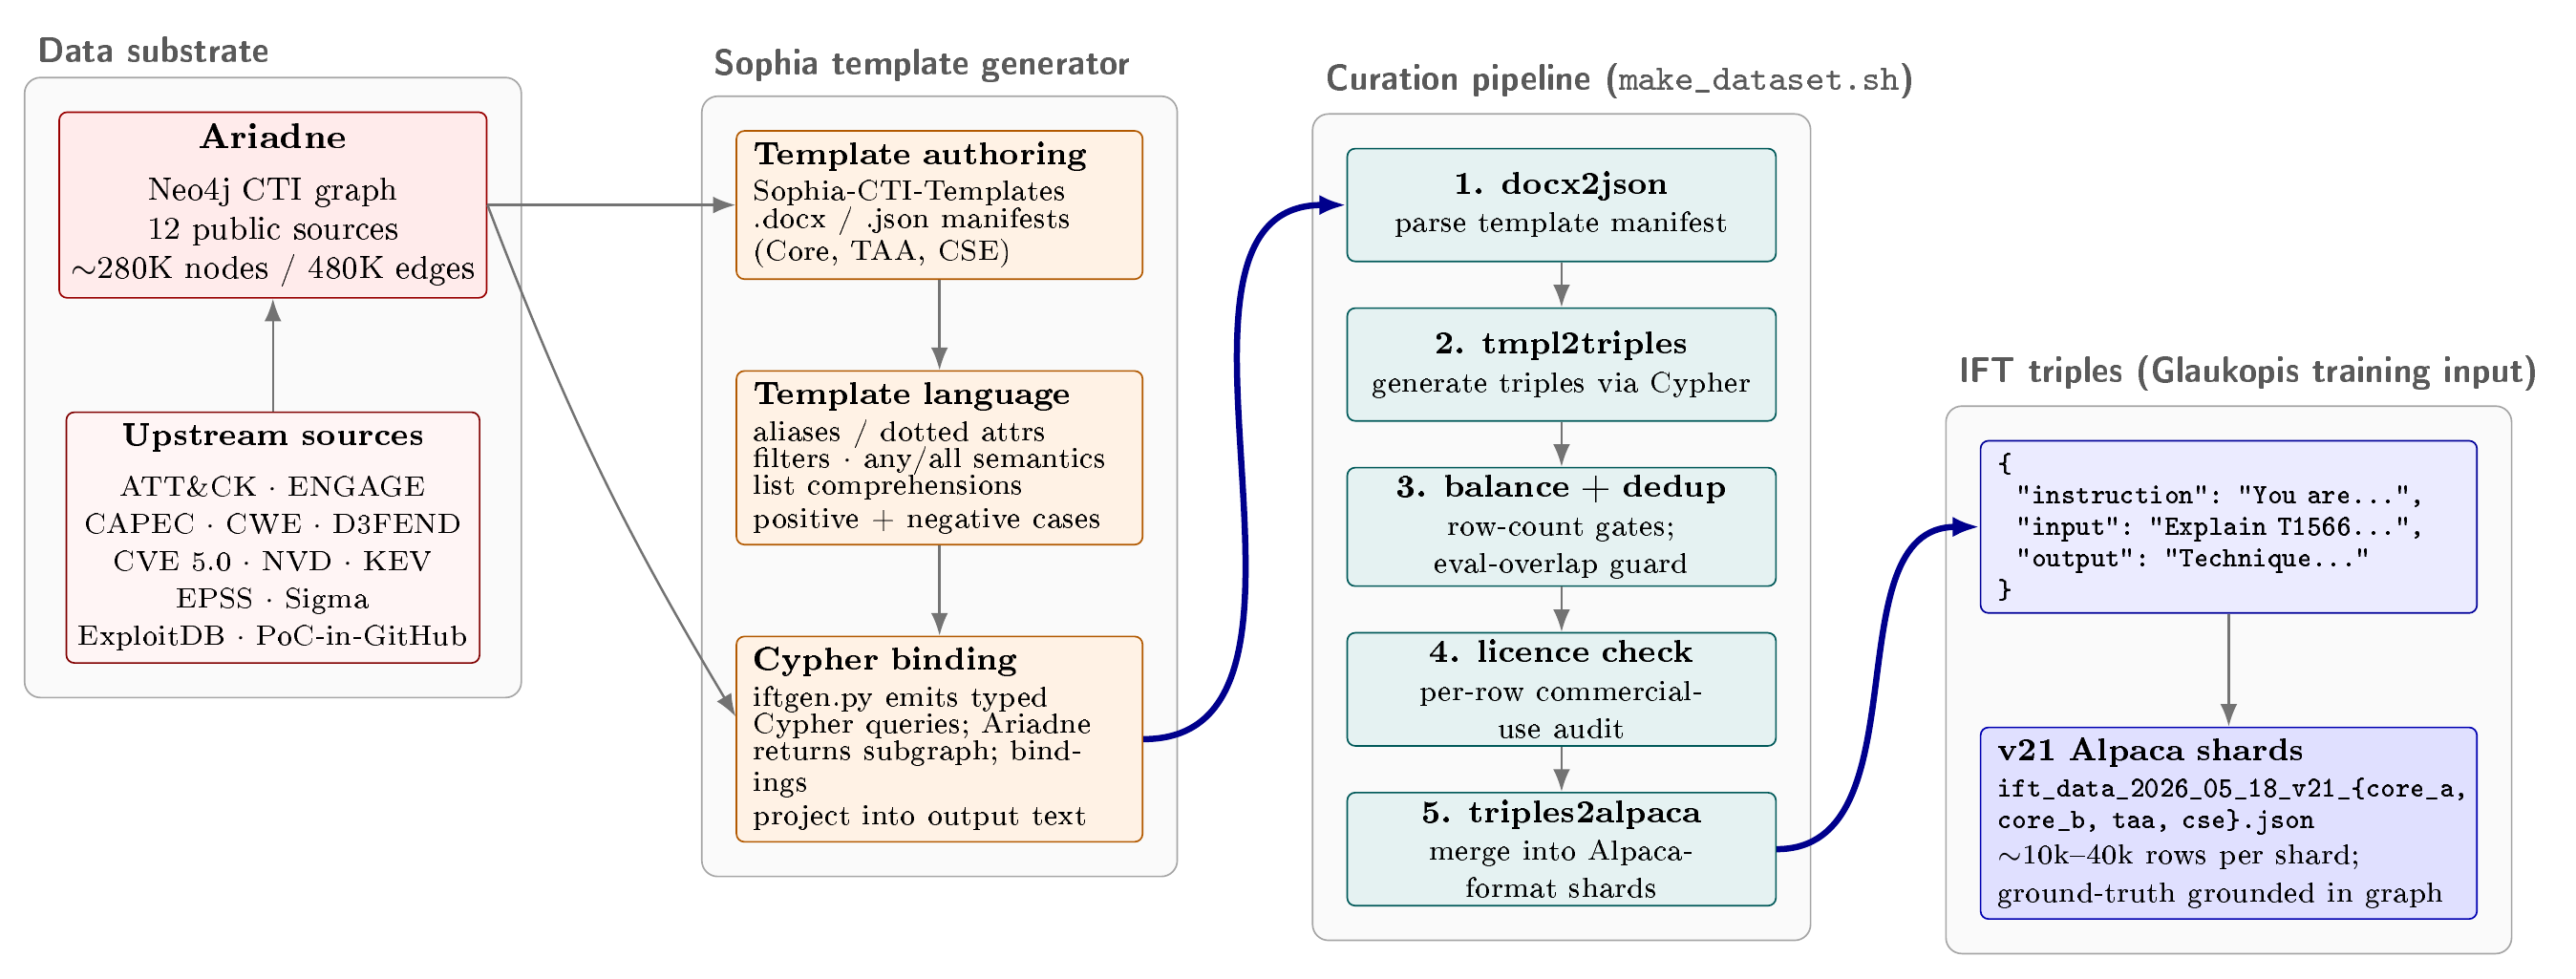
\includegraphics[width=\textwidth]{figures/glaukopis_sophia_flow.png}
\caption[]{\textbf{Sophia template generation and v21 data flow.} The upstream public CTI sources (left) are ingested into the Ariadne Neo4j graph. Sophia (centre-left) authors templates in three artefacts---template manifests (.docx/.json), the template language, and the Cypher binding step in \texttt{iftgen.py}---each of which compiles graph queries into natural-language output. The v21 curation pipeline (\hfid{make_dataset.sh}, centre-right) runs five steps in order: parse the template manifest, generate triples via Cypher, balance and dedup the corpus against the row-count gates and the eval-overlap guard (Appendix~\ref{app:contamination}), check per-row licence compliance, and merge the per-template files into Alpaca-format shards. The output (right) is the set of Alpaca-format IFT shard files (\texttt{ift\_data\_2026\_05\_18\_v21\_\{core\_a, core\_b, taa, cse\}.json}) consumed directly by the chained-IFT training stages (Section~\ref{sec:glaukopis-sft}).}
\label{fig:sophia-flow}
\end{figure*}

Sophia's key properties as a generator---taken collectively from the design document and its current implementation---are:

\begin{itemize}
  \item \textbf{CTI source coverage.} Sophia binds against the same twelve sources ingested by Ariadne (Section~\ref{sec:ariadne}), grouped for template-authoring purposes into three categories: (1) structural/graph sources (MITRE ATT\&CK, CVE, CAPEC, CWE, MITRE ENGAGE, EPSS, CISA KEV, D3FEND), bound directly via Cypher; (2) LLM-assisted sources (Sigma rules, MITRE CAR, Wazuh rules), where natural-language fields are augmented by LLM extraction before being merged into the graph; and (3) proprietary sources (e.g., Flashpoint Ignite) where licensed feeds are normalized into the same node and edge schema.
  \item \textbf{Triple format and serialization.} Each generated data point is a three-field record with \texttt{instruction}, \texttt{input}, and \texttt{output} keys in standard Alpaca format: the instruction specifies the role and style (e.g., ``You are a cyber security expert that gives precise responses to complex CTI questions''), the input is the user-facing CTI query, and the output is the ground-truth answer materialized from the CTI graph.
  \item \textbf{Template language.} Templates provide a high-level, declarative way to bind CTI graph nodes and produce triples. They support aliases for CTI types; attribute access through nested properties; filters with equality, inequality, and any/all semantics on list-valued properties; local variables bound to nodes; random selection from lists; list-comprehension-like constructs that expand relationships into output lists; invisible sections that establish bindings and constraints without appearing in surface text; and source disambiguation via a \verb|source#type| prefix (e.g., \verb|attck#attack-pattern| versus \verb|capec#attack-pattern|) \cite{cardei2025ift}.
  \item \textbf{Positive and negative examples.} The template language explicitly supports negative constraints (mitigations that do \emph{not} mitigate a technique, data components that do \emph{not} detect a technique used by a malware family), enabling systematic generation of hard negatives that teach models what does \emph{not} follow from the CTI graph.
  \item \textbf{Cross-source reasoning templates.} Example templates compose multi-hop reasoning chains: given a CVE description, identify the corresponding CWE weakness, then find a CAPEC attack pattern with high likelihood of attack using that weakness, then find an ATT\&CK technique that implements that attack pattern---each hop a typed query in Ariadne.
  \item \textbf{Incremental and time-windowed generation.} Sophia accepts version and date filters at both document and concept level: per-source version ranges and last-modified intervals can be specified in the job configuration, and relationships are only used if at least one endpoint and the relationship itself fall within those windows. This is what lets the training corpus track the threat landscape as new CTI material is ingested into Ariadne.
\end{itemize}

Operational details of the Sophia pipeline---the three-step \hfid{make_dataset.sh} workflow, the concrete template-syntax example, the active v21 template vintage at \hfid{templates/05182026/}, and the schema-validation tooling---are described in Section~\ref{sec:glaukopis-template} where they sit alongside the IFT chain that consumes them.

Conceptually, the Ariadne + Sophia pairing is a symbolic counterpart to the LLM-assisted instruction pipelines used in CyberPal and SEvenLLM: where CyberPal synthesizes security instructions from unstructured sources using LLMs and human experts \cite{levi2024cyberpal,levi2025toward}, Athena uses a declarative template language over a typed CTI graph to generate strongly grounded and precisely controllable instruction triples.

\subsection{CTI Knowledge Graphs and LLMs}
\label{sec:cti-kg-llms}

Recent work shows that LLMs and CTI knowledge graphs are synergistic. Various efforts use LLMs to extract triples from CTI text and populate knowledge graphs, then perform link prediction and reasoning over those graphs to produce actionable recommendations \cite{fieblinger2024kg,zhang2023cyberkg,wu2022opencykg,yu2024ctikg,zhao2024kctiaa}. Other systems build CTI-KGs directly from ATT\&CK, CVE, threat reports, and open sources, then query them using LLMs or hybrid systems for tasks such as threat hunting and reporting.

The Ariadne + Sophia design follows a complementary pattern: \emph{knowledge graph $\rightarrow$ templates $\rightarrow$ IFT triples $\rightarrow$ SLM}, with AthenaBench serving as a \emph{knowledge graph $\rightarrow$ evaluation tasks} pipeline on the evaluation side. This alignment is central to the next section.

\section{Glaukopis: A Chained-IFT Pipeline for Athena-CTI-LLM}
\label{sec:glaukopis}

Glaukopis is the template-based chained instruction fine-tuning (IFT) pipeline used to produce the Athena-CTI-LLM family of cyber security expert small language models. It is the concrete instantiation of the design principles surveyed in earlier sections: a CTI knowledge graph drives a template generator (Section~\ref{sec:cti-kg}); the generator emits IFT triples that are sharded into purpose-built training datasets; those datasets feed a multi-stage chained-IFT recipe (Section~\ref{sec:intro-chained-sft}); and the resulting checkpoints are evaluated against a portfolio of cyber security benchmarks (Section~\ref{sec:benchmarks}). This section describes each of these elements and how they fit together.

\subsection{Template-Based IFT: Sophia as the Training-Data Substrate}
\label{sec:glaukopis-template}

The Glaukopis training corpus is produced entirely by \textbf{Sophia} (\hfid{tmpl_gen}), the graph-template generator introduced in Section~\ref{sec:ariadne-templates}, operating against the Ariadne CTI substrate (Section~\ref{sec:ariadne}). This subsection covers the operational side of Sophia---the pipeline shape, the template-language surface syntax, the Alpaca output format, the active v21 vintage, and the schema-validation tooling---and the scientific properties of the template-driven IFT corpus that motivate its use as the substrate for every Glaukopis SFT stage.

\subsubsection*{Pipeline shape}
Sophia is a three-step pipeline driven by a single wrapper script, \hfid{data_generation/make_dataset.sh}, that runs end-to-end from authored templates to a Glaukopis-ready dataset:

\begin{enumerate}
  \item \texttt{docx2json.sh}---extracts templates from the authoring format (Word \texttt{.docx} or JSON) into a structured intermediate JSON. Templates can be authored in either form: each \texttt{.docx} paragraph encodes one template with inline \texttt{Id Instruction: \ldots Question: \ldots Answer: \ldots} markers, or each JSON object carries explicit \texttt{id}, \texttt{instruction}, \texttt{question}, \texttt{answer} fields.
  \item \texttt{tmpl2triples.sh}---reads the template JSON, opens a Bolt connection to Ariadne using the credentials in \hfid{neo4j-local-config.json}, issues the implied Cypher queries for each template, and emits per-template triple files in the configured results directory. A \hfid{_results-report.json} summary captures \hfid{failed_count} together with per-template generation counts so authors can diagnose binding failures.
  \item \texttt{triples2alpaca.sh}---merges all per-template triple files into a single Alpaca-format JSON dataset suitable as direct input to the IFT chain.
\end{enumerate}

The configurable knobs of the wrapper are a per-template generation ceiling (\hfid{count_limit}, default 10) controlling how many distinct bindings are sampled per template at the docx-to-JSON stage, and a maximum triple count (\hfid{count_max}, default 2{,}000) controlling the upper bound on triples emitted per template at the generation stage. These knobs are the per-stage shard-sizing controls used by the v21 build recipe in Section~\ref{sec:glaukopis-v21-templates}.

\subsubsection*{Template syntax}
A Sophia template binds graph nodes to local aliases, references their typed properties through dotted attribute access, and produces natural-language output containing the resolved values. A representative template (excerpted from the v21 manifest) reads:

\begin{quote}\scriptsize\ttfamily\sloppy\setlength{\rightskip}{0pt plus 2em}\noindent
M.1 Instruction: You are a cyber security expert that has been trained to give precise responses to complex CTI questions. You work in a SOC protecting data for enterprise customers.\\
Question: Explain ATT\&CK technique \{ap:attack-pattern.name\} (\{ap.id\}) and how it is used.\\
Answer: Technique \{ap.name\} (\{ap.id\}) is described as follows: \{ap.description\}. It is commonly observed across \{ap.x\_mitre\_platforms\}.
\end{quote}

Here \verb|{ap:attack-pattern.name}| introduces \texttt{ap} as a local alias for an ATT\&CK attack-pattern node and emits its \texttt{name} property; subsequent references \verb|{ap.id}|, \verb|{ap.description}|, and \verb|{ap.x_mitre_platforms}| reuse the same binding and emit additional properties of the same node. The full language adds relationship traversal (\verb|{var1.rel>TargetType.property}|), filters and any/all semantics on list-valued properties, list-comprehension constructs that expand relationships into output lists, invisible sections that establish bindings without producing surface text, and source-disambiguating prefixes (\verb|attck#attack-pattern| vs.\ \verb|capec#attack-pattern|). The detailed grammar is documented in Cardei's IFT design document \cite{cardei2025ift}.

\subsubsection*{Output format}
Each row of the Sophia output file is a three-key JSON object in standard Alpaca format, with \texttt{instruction} carrying the system role, \texttt{input} carrying the question derived from the template, and \texttt{output} carrying the answer materialized from the graph:

\begin{quote}\scriptsize\ttfamily\sloppy\setlength{\rightskip}{0pt plus 2em}\noindent
\{\\
\hspace*{1em}"instruction": "You are a cyber security expert\ldots",\\
\hspace*{1em}"input": "Explain ATT\&CK technique Phishing (T1566) and how it is used.",\\
\hspace*{1em}"output": "Technique Phishing (T1566) is described as follows: Adversaries may send phishing messages to gain access to victim systems. It is commonly observed across Windows, macOS, Linux."\\
\}
\end{quote}

The Alpaca shape is the canonical SFT input format used by LlamaFactory, AutoTrain, and the related open-source SFT tooling that the Glaukopis training scripts wrap; no further reformatting is required between Sophia output and SFT consumption.

\subsubsection*{Active vintage and provenance}
The active template vintage at the time of writing is \textbf{v21}, residing under \hfid{tmpl_gen/templates/05182026/} as three manifests---a Core manifest, a TAA manifest, and a CSE manifest---feeding the four-stage chained-IFT recipe of Section~\ref{sec:glaukopis-sft}. The v21 vintage is a strict-reproducibility experiment forked from the v18.1 vintage; the templates and per-stage row-count gates are byte-identical to v18.1, with only dataset names and Hugging Face push targets changed (Section~\ref{sec:glaukopis-v21-templates}).

\subsubsection*{Schema-validation tooling}
A separate \hfid{schema-test/} module accompanies Sophia and operates against the same Ariadne instance: it auto-generates test templates from a target CTI schema XLSX (\hfid{make-test-templates.sh}), runs them through the triple-generation engine (\hfid{test-CTI-schema.sh}), and emits a results report that flags any node label, property, or relationship that is referenced by a template but absent from the deployed graph. This is the mechanism by which Ariadne schema drift (e.g., a renamed property in a refreshed source) is detected before it can silently break template-generated training rows.

\subsubsection*{Scientific properties of template-driven IFT}
Sophia's design properties translate into several scientific advantages that motivate its use as the substrate for every Glaukopis SFT stage relative to purely LLM-generated instruction datasets:

\begin{itemize}
  \item \textbf{Ground-truth faithfulness.} Answers are computed directly from an authoritative CTI graph, reducing hallucinations and inconsistencies in training labels relative to instruction sets generated by an LLM acting as both author and oracle.
  \item \textbf{Explicit coverage control.} Templates can be designed to cover specific combinations of entities (e.g., CAPEC patterns affecting memory resources and their detection methods) or relationships (e.g., malware using two techniques on Linux), and per-template coverage fractions and count limits control dataset size and diversity \cite{cardei2025ift}.
  \item \textbf{Rich negative examples.} Inequality constraints and relationship filters enable systematic generation of hard negatives such as mitigations that do \emph{not} address a technique or data components that do \emph{not} detect any technique used by a malware family, exercising the model's ability to discriminate rather than simply complete.
  \item \textbf{Auditability and explainability.} Every Alpaca row maps to a specific template plus a specific graph binding; security experts can audit individual training rows by re-running the implied Cypher query, and changes to a template propagate deterministically to all rows it produced.
  \item \textbf{Incremental refresh.} Version and date filters allow periodic regeneration of updated IFT corpora as CTI sources evolve, paralleling AthenaBench's dynamic evaluation but on the training side \cite{cardei2025ift,alam2025athenabench}.
\end{itemize}

These properties together support a refreshable training loop in which new CTI material in Ariadne, new templates in Sophia, regenerated dataset shards, re-run SFT stages, and benchmark-driven feedback are all separable operations rather than a single monolithic retrain. The v21 vintage represents one concrete instantiation of this loop; the next vintage will refresh against an updated Ariadne snapshot and is expected to incorporate seed-pinning fixes to the substrate sampler discussed in Section~\ref{sec:glaukopis-v21-templates}.

\paragraph{Status.}
Sophia is in active development. Template syntax, parser behavior, and schema-test tooling may evolve as the CTI graph and the v21+ training pipeline mature; the descriptions in this section reflect the implementation as of the v21 vintage.

\subsection{Comparison with IBM's CyberPal and Other Instruction Pipelines}
\label{sec:glaukopis-vs-cyberpal}

The Athena approach is conceptually close to SecKnowledge/CyberPal, but with a different emphasis:

\begin{itemize}
  \item \textbf{CyberPal / SecKnowledge.} Uses expert-defined schemas and a pipeline combining LLMs and scripts to synthesize instructions from CTI sources and detection artifacts (e.g., Sigma rules), emphasizing human-curated ``expert instruction patterns'' and LLM-assisted generation, including CoT answers in SecKnowledge~2.0 \cite{levi2024cyberpal,levi2025toward}.
  \item \textbf{Sophia over Ariadne.} Uses a symbolic template language compiled into Cypher queries against the Ariadne CTI graph, producing triples that are guaranteed consistent with the knowledge graph, with strong use of cross-schema constraints and negative examples, and built around incremental, configuration-driven generation \cite{cardei2025ift}.
\end{itemize}

The two approaches are complementary. CyberPal demonstrates the effectiveness of expert instruction schemas and CoT enrichment in achieving high cyber security performance, especially in SLMs. The Ariadne + Sophia pairing provides precise and reproducible control over content generation aligned with CTI schemas and knowledge-graph structure, potentially feeding into similar CoT-enriched pipelines (e.g., by later adding CoT rationales using LLMs on top of graph-derived answers).

\subsection{The v21 Template-Generation Vintage}
\label{sec:glaukopis-v21-templates}

The Glaukopis IFT chain consumes training data produced by a versioned template-generation vintage. The active vintage at the time of writing is \textbf{v21} (template directory \hfid{tmpl_gen/templates/05182026/}), which is the configuration used for all hyperparameters, dataset structure, and results discussed in the rest of this section. This subsection describes the v21 template-generation flow---how Ariadne (Section~\ref{sec:ariadne}) is projected through three template manifests into the seven dataset shards consumed by the four-stage IFT chain (Section~\ref{sec:glaukopis-sft})---and the reproducibility and lineage discipline that produced it.

Figure~\ref{fig:glaukopis-v21-flow} summarizes the end-to-end pipeline. Ariadne feeds three template manifests: a \emph{Core} manifest covering Stages~1 and~4, a \emph{TAA} manifest covering Stage~2, and a \emph{CSE} manifest covering Stage~3. Each manifest is processed by the same three-step \hfid{make_dataset.sh} pipeline---\texttt{docx2json} extracts templates from their authoring format, \texttt{tmpl2triples} drives the IFT-generation engine against the Neo4j graph, and \texttt{triples2alpaca} merges per-template triple JSON files into a single Alpaca-format dataset (with \texttt{instruction}, \texttt{input}, and \texttt{output} keys mapping to system, prompt, and response respectively). The result is four production training shards plus three matched validation shards, all template-baked and therefore architecture-independent: a single set of seven JSON files feeds every base-model port of the v21 recipe.

\begin{figure*}[t]
\centering
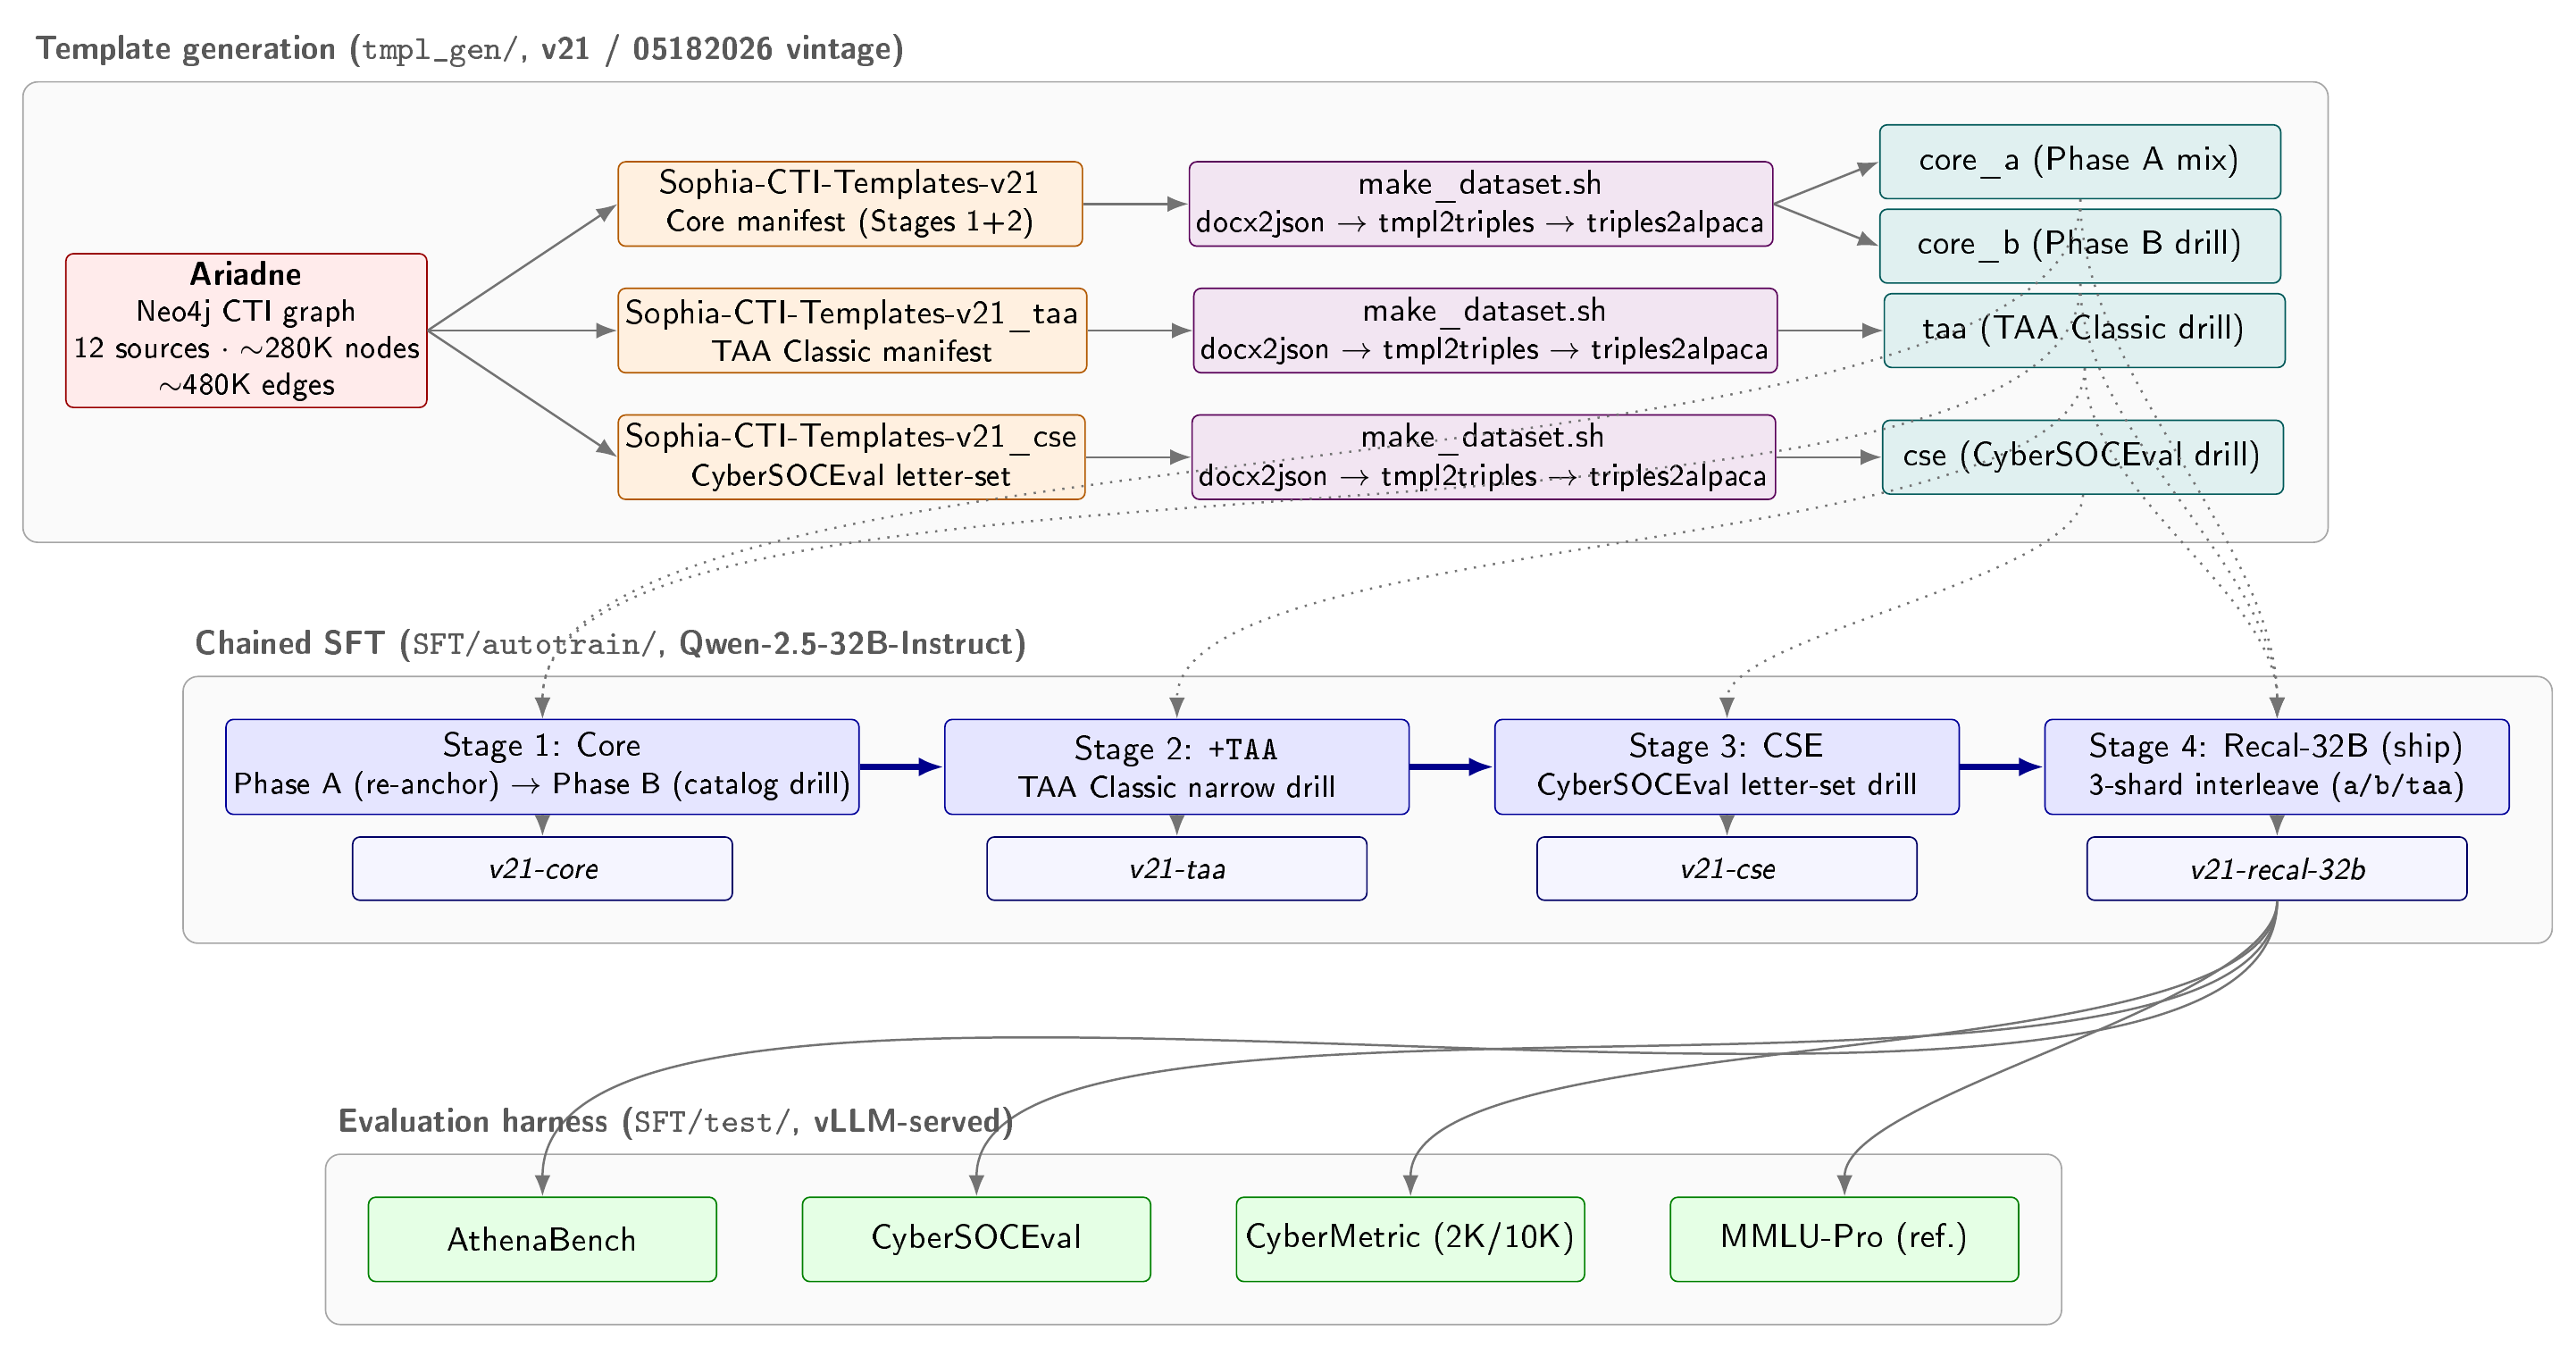
\includegraphics[width=\textwidth]{figures/glaukopis_v21_flow.png}
\caption[]{\textbf{Glaukopis v21 end-to-end flow.} Ariadne (Section~\ref{sec:ariadne}), the Athena Neo4j CTI substrate, feeds three v21 template manifests---Core, TAA, and CSE---each processed by the \hfid{make_dataset.sh} pipeline into Alpaca-format dataset shards. Four production shards (\hfid{core_a}, \hfid{core_b}, \texttt{taa}, \texttt{cse}; matched validation shards omitted for clarity) drive the four-stage chained-IFT recipe targeting Qwen-2.5-32B-Instruct, producing the cumulative \hfid{v21-core}, \hfid{v21-taa}, \hfid{v21-cse}, and ship \hfid{v21-recal-32b} checkpoints. Dotted arrows mark which shards feed which stages; Stage~4 re-uses Core-A, Core-B, and TAA as a three-shard interleaved touch-up. Each pushed checkpoint is evaluated against the AthenaBench, CyberSOCEval, CyberMetric, and MMLU-Pro suites under a vLLM-served harness.}
\label{fig:glaukopis-v21-flow}
\end{figure*}

\paragraph{Reproducibility provenance.}
v21 is a strict reproducibility experiment on top of a predecessor vintage v18.1. The three Sophia-CTI template manifests, the row-count gate JSONs, and the per-stage count limits are \texttt{shasum}-verified byte-identical to their v18.1 sources; only dataset names, build-directory names, and Hugging Face push targets change between the two vintages. The v21 sign-off gate was that the post-Core checkpoint would land within $\pm 1.5$ percentage points of the v18.1 Core peak on every benchmark axis. The Total Score landed inside that band, but two per-axis sub-scores (ATE and RCM) drifted outside it, with the same shape that the intermediate v19 and v20 vintages had previously shown against v18.1. The most parsimonious explanation, given that the recipe-side inputs are byte-identical, is data-build non-determinism in the substrate sampler, dedup tiebreaks, and shuffle seeding inside \hfid{make_dataset.sh}---a hypothesis confirmed by the fact that pinning the Neo4j read order and seeding the substrate sampler is the next-vintage research direction. The lineage discipline is in our judgement itself a contribution: by carrying byte-identical templates and gates forward across vintages, the Glaukopis pipeline isolates recipe drift from data-layer drift as separable failure modes, and provides a falsification matrix against which future vintages can be evaluated.

\paragraph{The off-plan Recalibrate stage.}
The v21 plan as originally specified was a three-stage chain (Core $\to$ +TAA $\to$ CSE). A recurring pattern observed across v18.1, v19, v20, and v21 chains is that Stage~3's narrow CyberSOCEval-letter-set drill reliably trades approximately ten percentage points of VSP for the CyberSOCEval-Malware lift it is designed to produce. To recover the VSP regression without sacrificing the Stage~3 gains, an off-plan fourth stage---\emph{Recalibrate}---was added as a three-shard interleaved touch-up over Core-A, Core-B, and TAA. At the 14B base scale, a single Recalibrate recipe (1e-6 LR, $0.25 / 0.40 / 0.35$ interleave probabilities, \hfid{--max-samples 2400}) cleanly recovers VSP. At the 32B base scale, the same recipe sits at the \hfid{adamw_8bit} optimizer noise floor and drifts VSP the wrong way; the recipe was therefore re-tuned (3e-6 LR, $0.15 / 0.60 / 0.25$ Phase-B-heavy mix, \hfid{--max-samples 3600}) to expose more VSP/RMS catalog per interleaved row while holding step count and wall-time constant. The 32B Stage~4 split is the basis of the ship checkpoint discussed in Section~\ref{sec:glaukopis-sft}.

\paragraph{Architecture ports.}
Stages 1 through 3 carry the same recipe byte-identically across all five base-model ports of v21: Qwen-2.5-32B-Instruct (canonical), Qwen-2.5-14B-Instruct, Foundation-Sec-8B, Llama-3.1-8B-Instruct, and Qwen3-30B-A3B-Thinking-2507 (a thinking-mode MoE). The fact that the same template-baked shards drive all ports is what makes cross-architecture comparison meaningful: any axis-level differences between checkpoints derived from different bases under the same recipe and same data are attributable to base-model differences rather than training-data drift. The Qwen3-MoE port is also the first port to exercise a thinking-on / thinking-off A/B at serve time, exposing the SFT contribution to no-trace inference behavior separately from the base model's reasoning gain. Stage 4 is the only stage where the recipe does not carry identically across architectures: at the 32B dense scale the Phase-B-heavy 3e-6 LR variant is required (as discussed above), and on the Qwen3-MoE port Stage~4 closed without a beat against \hfid{v21-cse} on either Stage-4 variant, so the on-chain ship for that port is \hfid{v21-cse}. Table~\ref{tab:base-models} lists the five baseline instruct models used as Stage-0 inputs, with the canonical Hugging Face identifiers used in the evaluation harness and on the Hugging Face Hub.

\begin{table*}[t]
\centering
\caption{Baseline instruct models targeted by the v21 architecture ports. The canonical Hugging Face identifiers are used verbatim in the evaluation-harness model registry and in the cross-architecture port launchers under \texorpdfstring{\hfid{SFT/autotrain/}}{SFT/autotrain/}. The dense Qwen-2.5-32B-Instruct is the canonical Stage-0 base for the ship checkpoint reported in Section~\ref{sec:results-headline}; the other four are cross-architecture ports of the same v21 chain.}
\label{tab:base-models}
\small
\setlength{\tabcolsep}{4pt}
\begin{tabular}{p{4.8cm} l l l}
\hline
\textbf{Canonical HF identifier} & \textbf{Family} & \textbf{Architecture} & \textbf{Role in v21} \\
\hline
\hfid{Qwen/Qwen2.5-32B-Instruct}             & Qwen 2.5             & 32B dense          & Canonical Stage-0 base (ship) \\
\hfid{Qwen/Qwen2.5-14B-Instruct}             & Qwen 2.5             & 14B dense          & Cross-architecture port \\
\hfid{Qwen/Qwen3-30B-A3B-Thinking-2507}      & Qwen 3 Thinking      & 30B MoE (A3B)      & MoE / thinking-mode port \\
\hfid{meta-llama/Meta-Llama-3.1-8B-Instruct} & Llama 3.1            & 8B dense           & Cross-architecture port \\
\hfid{fdtn-ai/Foundation-Sec-8B-Instruct}    & Foundation-Sec       & 8B dense           & Security-specialized base (Cisco) \\
\hline
\end{tabular}
\end{table*}

\subsection{The Glaukopis SFT Chain}
\label{sec:glaukopis-sft}

The Glaukopis IFT chain is a four-stage chain over Sophia-generated CTI instruction data, using standard supervised fine-tuning (SFT) on next-token cross-entropy at each stage. The canonical configuration targets Qwen-2.5-32B-Instruct as the base model and produces a sequence of four cumulative checkpoints---Core, +TAA, CSE, and Recalibrated-32B---of which the last is the production ship checkpoint. The same recipe ports byte-identically to four other base architectures (Qwen-2.5-14B-Instruct, Foundation-Sec-8B, Llama-3.1-8B-Instruct, and the Qwen3-30B-A3B-Thinking-2507 MoE), with only the base-model pointer and per-architecture memory flags changing between ports. The four-stage structure is itself the load-bearing element of the recipe; the per-stage details are described below.

\paragraph{Dataset shards.}
The chain consumes seven dataset shards produced by the template generator. The \textbf{Core-A} shard is a broad re-anchor mix combining knowledge-base, multiple-choice, threat-actor-attribution (TAA), SOC-style, CyberMetric-style, mitigation-strategy, and yes/no instruction families. The \textbf{Core-B} shard is an AthenaBench catalog drill targeting Risk Mitigation Strategy (RMS), Attack Technique Extraction (ATE), Vulnerability Severity Prediction (VSP), and Root Cause Mapping (RCM) tasks \cite{alam2025athenabench}. The \textbf{TAA} shard is a narrow drill on TAA Classic. The \textbf{CSE} shard is a CyberSOCEval letter-set drill, structured to exercise the format and reasoning pattern used by the CyberSOCEval malware and threat-intel test suites \cite{cybersoceval2025}. Three matched validation shards (\textbf{Core-Val}, \textbf{TAA-Val}, \textbf{CSE-Val}) hold out a per-axis slice (50 rows per shortname) for held-out evaluation during training. All shards are template-baked and therefore architecture-independent: a single set of seven JSON files feeds every base-model port.

\paragraph{Stage 1: Core (broad re-anchor + AthenaBench catalog drill).}
Stage 1 runs as two phases inside a single launcher, with only the final phase's merged checkpoint pushed. \emph{Phase A} is the broad re-anchor: it trains on the Core-A shard together with a general-purpose instruction mix (the Tülu-3 SFT mixture and an Alpaca-English demonstration set) at sequence length 8\,192, packing on, learning rate $1 \times 10^{-5}$, and effective batch size 16. The intent is to re-establish broad instruction-following behavior on top of a CTI vocabulary base. \emph{Phase B} drills on the Core-B AthenaBench-catalog shard at sequence length 16\,384 with packing off (so that long structured outputs are not truncated by packing boundaries), learning rate $5 \times 10^{-6}$, and effective batch size 8. The shorter, lower-LR Phase B is calibrated to imprint precise AthenaBench task structure on top of the broad foundation laid by Phase A, rather than to continue broad assimilation \cite{alam2025athenabench}. Together, Phase A and Phase B implement at fine granularity the principle from FLAN-T5 and ``Don't Stop Pretraining'' that broad domain exposure and narrow task supervision benefit from separate optimization regimes \cite{chung2022flant5,gururangan2020dontstop}.

\paragraph{Stage 2: +TAA narrow drill.}
Stage 2 takes the Core checkpoint as its base and trains on the TAA shard alone, at sequence length 4\,096, packing on, learning rate $5 \times 10^{-6}$, and effective batch size 16. The objective is to harden the model's TAA Classic performance without disturbing the broader catalog skills established in Stage 1.

\paragraph{Stage 3: CSE letter-set drill.}
Stage 3 takes the +TAA checkpoint and trains on the CSE shard at the same sequence length, packing, learning rate, and effective batch size as Stage 2. This stage is targeted preparation for the CyberSOCEval malware and threat-intelligence suites \cite{cybersoceval2025}, and is the point at which a known trade-off appears: lifting the CyberSOCEval axis through this drill comes at a measured cost to VSP performance from Stage 1's Phase B, which the next stage exists to recover.

\paragraph{Stage 4: Recalibrated touch-up (ship variant).}
Stage 4 is a three-shard interleaved touch-up trained off the Stage 3 (CSE) checkpoint with the explicit goal of recovering the VSP regression introduced by Stage 3 without losing Stage 3's CyberSOCEval gains. The ship variant trains on a Core-A / Core-B / TAA mix at relative sampling probabilities $0.15 / 0.60 / 0.25$ (i.e., Phase-B-heavy), using LlamaFactory's \hfid{interleave_under} mixing strategy with a 3\,600-row sample cap, at sequence length 16\,384, packing off, learning rate $3 \times 10^{-6}$, and effective batch size 8. The 14B-tuned variant of this recipe (lower learning rate, more balanced mixture, smaller sample cap) is retained as a recipe-provenance A/B against the ship-grade 32B recipe, but in the 32B-target chain it is the higher-LR, Phase-B-heavy variant that recovers VSP and tops the v21 evaluation leaderboard.

\paragraph{Cross-cutting training-system details.}
All four stages share the same systems-level configuration: bf16 mixed precision, DeepSpeed ZeRO-3 (with optional CPU offload), the \hfid{adamw_8bit} optimizer (mandatory at the 32B scale to fit activations), Liger kernels for fused attention paths, and gradient checkpointing on at 32B regardless of GPU count. The 8$\times$H100-80GB SXM topology is the canonical training target; 8$\times$H200-141GB SXM and 8$\times$RTX-PRO-6000-96GB are supported alternates. Effective batch size is held constant across launch topologies by auto-scaling gradient accumulation to GPU count.

\paragraph{Why four stages rather than one.}
The four-stage structure embodies the chained-IFT rationale from Section~\ref{sec:intro-chained-sft} in a CTI-specific form. Stages 1A and 1B separate broad domain absorption from precise structured-task imprinting, each at its own learning rate and packing regime \cite{gururangan2020dontstop,chung2022flant5}. Stages 2 and 3 carry out narrow drills against specific benchmark axes (TAA and CyberSOCEval respectively) without re-perturbing the broader skill set learned in Stage 1. Stage 4 is a recalibration step that recovers regressed axes (here, VSP) through controlled three-shard interleaving and a slightly higher learning rate, exploiting the fact that all template-generated shards remain available as training corpora throughout the chain. The result is a sequence of intermediate checkpoints---Core, +TAA, CSE, Recalibrated-32B---that can each be evaluated independently against the benchmark portfolio of Section~\ref{sec:benchmarks}, supporting controlled per-stage ablation in addition to producing a single ship checkpoint. This per-stage observability is itself a benefit of the chained structure: any axis-level regression observed at evaluation time is attributable to a specific stage and a specific dataset shard, and can be addressed by re-running only the affected stages rather than the full pipeline.

\subsection{Evaluation Harness}
\label{sec:glaukopis-eval}

Each pushed checkpoint in the Glaukopis chain is evaluated against the portfolio described in Section~\ref{sec:benchmarks}, consisting of \textbf{AthenaBench} (the six CTI tasks: CKT/MCQ, RCM, VSP, ATE, TAA Classic and Canonical, and RMS) \cite{alam2025athenabench}; \textbf{CyberSOCEval} (the malware and threat-intelligence test suites) \cite{cybersoceval2025}; \textbf{CyberMetric} at the 2\,000- and 10\,000-question tiers \cite{tihanyi2024cybermetric}; and \textbf{MMLU-Pro} as a decoupled general-intelligence reference. Serving is via vLLM in an OpenAI-compatible configuration; the same alias-keyed harness scores public baselines through hosted inference providers for direct comparison. Per-task token and wall-clock usage is captured so that benchmark sweeps are accompanied by a cost summary covering both API and local-GPU compute, which lets evaluation cost be reported alongside accuracy as a first-class metric.

The mapping between training stages and evaluation suites is deliberate: AthenaBench RMS/ATE/VSP/RCM are exercised by Stage 1 Phase B's Core-B shard; AthenaBench TAA Classic and TAA Canonical are exercised by Stage 2; CyberSOCEval malware and threat-intel reasoning are exercised by Stage 3; CyberMetric and the AthenaBench MCQ axis are exercised primarily by Stage 1 Phase A's Core-A shard. The Stage 4 recalibration is designed not to alter this mapping but to recover any axis that has regressed across the prior stages, with the 32B-tuned, Phase-B-heavy mixture specifically chosen to restore VSP without sacrificing CyberSOCEval performance. MMLU-Pro is run on a separate session so that suite scope stays decoupled from CTI scoring: it is reported as a sanity check on general capability rather than as a target for optimization.

\subsection{Toward Cyber Security Expert Small Language Models}
\label{sec:glaukopis-expert-slm}

Bringing together the elements above, an end-to-end cyber security expert SLM pipeline of the kind exemplified by Glaukopis can be summarized as:

\begin{enumerate}
  \item \textbf{CTI graph construction.} Continuously ingest and normalize CTI sources (ATT\&CK, CVE, CAPEC, CWE, ENGAGE, ICS/OT sources, proprietary feeds) into a Neo4j or similar graph.
  \item \textbf{Template authoring.} CTI experts encode important reasoning patterns (knowledge recall, root cause mapping, severity estimation, attribution clues, mitigation reasoning) as templates in the Athena language.
  \item \textbf{IFT generation.} Run the generation tool with version and date constraints aligned to a training window, producing large, structured IFT datasets per task family \cite{cardei2025ift}.
  \item \textbf{Chained SFT.} Fine-tune SLMs (e.g., 8--32B open models) using a chain of stages as described in Section~\ref{sec:glaukopis-sft}, with the dataset-shard / stage mapping aligned to the benchmark portfolio.
  \item \textbf{Evaluation.} Benchmark models on AthenaBench, CyberSOCEval, CyberMetric, and complementary suites (CTIBench, SecEval, CyberBench, SEvenLLM-Bench) to assess generalization and compare with larger proprietary models \cite{alam2024ctibench,alam2025athenabench,hu2024seceval,liu2024cyberbench,ji2024sevenllm,tihanyi2024cybermetric,cybersoceval2025}.
  \item \textbf{Feedback and iteration.} Use benchmark error patterns to design new templates, adjust CTI graph coverage, or refine IFT data (e.g., adding more negative cases or multi-hop chains), and re-run only the affected SFT stages.
\end{enumerate}

This pipeline is closely aligned with IBM's vision of cyber security expert SLMs \cite{levi2024cyberpal,levi2025toward}, but anchored in Athena's graph-driven IFT, the chained-IFT recipe described above, and dynamic CTI benchmarking via AthenaBench and CyberSOCEval.


\section{Results}
\label{sec:results}

This section reports the evaluation of the v21 Glaukopis vintage against the benchmark portfolio of Section~\ref{sec:benchmarks}: AthenaBench (six tasks: CKT, ATE, RCM, RMS, VSP, and TAA, with TAA scored as the combined-form average across Classic and Canonical), CyberSOCEval (Malware-analysis and Threat-Intel-Reasoning subsets), CyberMetric at the 2\,000- and 10\,000-question tiers, and MMLU-Pro as a decoupled general-intelligence reference. All numbers in this section come from the same harness run (sweep dated 2026-05-24), use the same vLLM serving stack for local checkpoints, and use the same hosted-API endpoints for public-model baselines.

\subsection{Three Averaging Schemes and Why MMLU-Pro Is Reported Separately}
\label{sec:results-averaging}

Because the three CTI benchmarks differ substantially in their internal structure---AthenaBench has six tasks, CyberSOCEval has two, and CyberMetric has two tiers---there is no single canonical way to aggregate them into a summary number, and the choice of aggregation visibly changes the leaderboard. We therefore report three averages for every model:

\begin{itemize}
  \item \textbf{Avg CTI Benchmark Score.} The unweighted mean of three per-benchmark summaries: AthenaBench (combined), CyberSOCEval (combined), and CyberMetric (2K+10K average). Each benchmark contributes equal weight regardless of how many internal tests it contains. This is the closest analogue to how published leaderboards typically present cyber LLM results and is the score we use for cross-benchmark comparison.
  \item \textbf{Avg CTI Test Score.} The unweighted mean across the ten individual CTI tests---six AthenaBench tasks, two CyberSOCEval subsets, and the two CyberMetric tiers---giving each test equal weight. This view is sensitive to the internal structure of each benchmark: AthenaBench, with six tests, exerts more pull on the score than CyberSOCEval or CyberMetric, which have two tests each. It is the most informative when the goal is to compare aggregate per-task capability.
  \item \textbf{Avg Total Test Score (with MMLU-Pro).} The same per-test average as above, but extended to include MMLU-Pro. MMLU-Pro is a general-intelligence reference and is \emph{not} part of the CTI use case we ultimately care about; we report this third average chiefly to quantify how much general capability each SFT run has traded away for CTI specialization---a \textit{general-knowledge erosion} diagnostic (often called \textit{catastrophic forgetting} in the SFT literature) rather than a target for optimization.
\end{itemize}

The three averages tell complementary stories. The per-benchmark average is the most charitable view for SFT models, because it rewards strong performance on benchmarks whose internal structure aligns with the training data (here, AthenaBench). The per-test average reweights toward AthenaBench's six tasks but is invariant to how those tasks are pooled, making it the most apples-to-apples cross-architecture metric. The MMLU-Pro-augmented average is informative only as a counterpoint: SFT'd models systematically lose MMLU-Pro relative to their bases, and the magnitude of that loss is a useful diagnostic for the cost of specialization.

A per-evaluation cost analysis accompanies the accuracy results and is reported in Section~\ref{sec:results-cost}. We use a uniform measurement methodology---published per-1K-token rate cards for hosted-API checkpoints, and wall-clock seconds at \$2.50/GPU-hour on a 2$\times$H100 reference host for locally-served vLLM checkpoints---so that the dollar cost of a full-suite evaluation pass can be reported alongside the accuracy number for every model. Cost is the second dimension on which Glaukopis differentiates from frontier reference points.

\subsection{Headline Comparison: v21 Ship Checkpoint vs.\ Frontier Reference Points}
\label{sec:results-headline}

Table~\ref{tab:results-headline} compares the Glaukopis v21 ship checkpoint, \hfid{athena-cti-sft-qwen25-32b-v21-recal-32b}, against its base instruct model and against six frontier-class reference points spanning the major proprietary and open-weights frontier families. All three averages are reported alongside the underlying per-benchmark scores. Three observations:

\begin{enumerate}
  \item \textbf{Chained SFT adds 7.3 points of average CTI benchmark capability over the base Qwen-2.5-32B-Instruct} (59.0 $\to$ 66.3) without changing the parameter count or runtime footprint. On the per-test average the lift is even larger (49.6 $\to$ 62.9, +13.3 points), because the per-test average gives full weight to AthenaBench's six tasks, on which the chain is explicitly trained. The largest single-axis lift is on AthenaBench combined (44.2 $\to$ 66.5; +22.3 absolute).
  \item \textbf{The ship checkpoint approaches frontier-class CTI performance.} On Avg CTI Benchmark Score the v21 ship sits within 4--7 points of the leading frontier models (GPT-5.5 at 72.9, DeepSeek-V4-Pro at 70.4, Gemini-3-Flash-Preview at 69.8), and is closely competitive with mid-tier frontier offerings (GPT-5.2 at 67.5, DeepSeek-v3.2-Exp at 66.0). On Avg CTI Test Score the same pattern holds (62.9 vs.\ leaders at 67--73). It is competitive with Gemini-2.5-Flash on both averages despite the substantial parameter-count gap.
  \item \textbf{General-knowledge erosion in the MMLU-Pro dimension is real, but not unique to Glaukopis and not a target for optimization.} MMLU-Pro drops from 69.0 (Qwen-2.5-32B-Instruct base) to 57.4 (v21 ship), an 11.6-point absolute regression that reflects the well-known cost of domain specialization. The Avg Total Test Score (with MMLU-Pro) figure makes this explicit: the v21 ship at 62.8 trails GPT-5.5 (76.9) by a wider margin on this composite than on either CTI-only average. The phenomenon is conventionally labeled \textit{catastrophic forgetting} in the SFT literature; we prefer the more accurate term \textit{general-knowledge erosion}, because what occurs in practice across our ports is a graded, parameter-count-dependent degradation of out-of-domain capability rather than a sudden, total loss. The graded pattern is visible in Table~\ref{tab:results-architectures}: the 8B ports lose 17.6--20.6 MMLU-Pro points, the 14B port loses 13.9, the dense 32B port loses 11.6, and the Qwen3-MoE port (largest active-parameter count among ports we ran) loses the most at 24.6---an outlier driven by the MoE architecture rather than by the base-model size. The dominant trend among dense ports is that larger base models erode less under the same recipe. Because MMLU-Pro is not part of the CTI use case we ultimately care about, this erosion is reported as a diagnostic rather than treated as a metric to optimize against; we discuss possible mitigations, including the option of moving to a larger base model, in Section~\ref{sec:open-challenges}.
\end{enumerate}

\begin{table*}[t]
\centering
\caption{Headline results: Glaukopis v21 ship checkpoint vs.\ base model and frontier reference points. Three averages are reported per the schemes defined in Section~\ref{sec:results-averaging}: \textbf{Avg CTI Bench} (3 benchmarks, equal weight), \textbf{Avg CTI Test} (10 CTI tests, equal weight), and \textbf{Avg Total (w/MMLU)} (10 CTI tests plus MMLU-Pro). All numbers from the 2026-05-24 evaluation sweep. AB Avg II is the AthenaBench composite using the 50/50 TAA Classic+Canonical blend.}
\label{tab:results-headline}
\small
\setlength{\tabcolsep}{4pt}
\begin{tabular}{lcccccccc}
\hline
\textbf{Model} & \textbf{Type} & \textbf{Avg CTI} & \textbf{Avg CTI} & \textbf{Avg Total} & \textbf{AB Avg} & \textbf{CSE} & \textbf{CM} & \textbf{MMLU-} \\
               &               & \textbf{Bench}   & \textbf{Test}    & \textbf{(w/MMLU)}  & \textbf{II}    & \textbf{comb} & \textbf{avg} & \textbf{Pro} \\
\hline
GPT-5.5                                  & Frontier  & 72.9 & 73.5 & 76.9 & 77.0 & 48.3 & 93.3 & 88.3 \\
DeepSeek-V4-Pro                          & OS-PT     & 70.4 & 67.9 & 69.6 & 67.2 & 52.2 & 91.8 & 79.1 \\
Gemini-3-Flash-Preview                   & Frontier  & 69.8 & 68.4 & 71.7 & 69.3 & 48.1 & 92.1 & 89.2 \\
GPT-5.2 (reasoning=medium)               & Frontier  & 67.5 & 65.0 & 67.0 & 63.8 & 46.8 & 91.8 & 81.3 \\
DeepSeek-v3.2-Exp                        & OS-PT     & 66.0 & 62.2 & 63.9 & 59.0 & 47.2 & 91.7 & 82.5 \\
\textbf{v21-recal-32b (ship)}            & SFT       & \textbf{66.3} & \textbf{62.9} & \textbf{62.8} & \textbf{66.5} & 42.6 & 89.8 & 57.4 \\
v21-cse                                  & SFT       & 65.8 & 62.4 & 62.2 & 66.6 & 42.0 & 88.8 & 54.2 \\
v21-recalibrate (14B-recipe)             & SFT       & 65.9 & 62.4 & 62.2 & 65.9 & 42.4 & 89.2 & 54.6 \\
Gemini-2.5-Flash                         & Frontier  & 63.4 & 57.9 & 59.8 & 53.1 & 46.2 & 91.0 & 82.1 \\
v21-core                                 & SFT       & 62.6 & 61.6 & 63.2 & 67.2 & 31.1 & 89.6 & 59.2 \\
v21-taa                                  & SFT       & 62.0 & 61.7 & 63.7 & 66.9 & 29.8 & 89.4 & 58.2 \\
Qwen2.5-32B-Instruct (base)              & Instruct  & 59.0 & 49.6 & 49.3 & 44.2 & 42.6 & 90.2 & 69.0 \\
\hline
\end{tabular}
\end{table*}

\paragraph{Why \texorpdfstring{\hfid{v21-recal-32b}}{v21-recal-32b} is the ship checkpoint, not \texorpdfstring{\hfid{v21-recalibrate}}{v21-recalibrate}.}
The two Stage-4 variants warrant brief comparison because they share the same Stage-3 parent (\hfid{v21-cse}) and differ only in the Stage-4 recipe. \hfid{v21-recalibrate} runs the 14B-tuned Stage-4 recipe verbatim on the 32B base (learning rate $1\times 10^{-6}$, balanced 0.25/0.40/0.35 interleave probabilities, \hfid{--max-samples 2400}); \hfid{v21-recal-32b} runs the recipe re-tuned for the 32B parameter scale (learning rate $3\times 10^{-6}$, Phase-B-heavy 0.15/0.60/0.25 mix, \hfid{--max-samples 3600}). On the headline aggregates the two variants are within 0.5 points of each other (Avg CTI Bench 66.3 vs.\ 65.9; Avg CTI Test 62.9 vs.\ 62.4), which on its own would not be enough to prefer one over the other. The deciding factor is per-axis: \hfid{v21-recal-32b} restores VSP to 77.8 against \hfid{v21-recalibrate}'s 75.7, and that VSP recovery is precisely what Stage~4 is for at the 32B scale (Section~\ref{sec:glaukopis-v21-templates}). The 14B-recipe variant sits at the \hfid{adamw_8bit} optimizer noise floor at 32B---enough to nudge most axes in the right direction, but not enough to recover the VSP regression introduced by Stage~3. \hfid{v21-recal-32b} is therefore the recommended ship checkpoint at the 32B scale, with \hfid{v21-recalibrate} retained on disk as the recipe-provenance A/B against it.

\subsection{Per-Stage Ablation: What Each SFT Stage Contributes}
\label{sec:results-per-stage}

Because the Glaukopis chain pushes a Hugging Face checkpoint after every stage, the per-stage contribution to each benchmark axis is directly measurable. Table~\ref{tab:results-per-stage} reports the AthenaBench axis breakdown for the Qwen-2.5-32B chain alongside the base model, decomposing how Core $\to$ +TAA $\to$ CSE $\to$ Recalibrate-32B accumulates capability.

The data confirm the design rationale of the chain (Section~\ref{sec:glaukopis-sft}):

\begin{itemize}
  \item \textbf{Stage 1 (Core) does most of the AthenaBench-catalog work.} The Phase~B catalog drill lifts ATE from 18.2 (base) to 67.2 (Core), RMS combined-f1 from 7.6 to 63.8, and RCM from 59.5 to 69.8. These are the gains the rest of the chain must preserve.
  \item \textbf{Stage 2 (+TAA) introduces meaningful Canonical-TAA capability.} TAA Canonical combined rises from 2.0 (base) and 18.4 (Core) to 36.8 at +TAA, the largest single-stage Canonical lift in the chain.
  \item \textbf{Stage 3 (CSE) lifts the CyberSOCEval axis} from 31.1 (Core) to 42.0 (CSE), a +10.9 absolute gain. The expected VSP trade-off is also visible: VSP drops from 83.1 (Core) to 78.9 (CSE), consistent with the regression pattern observed across v18.1, v19, v20, and v21 (Section~\ref{sec:glaukopis-v21-templates}).
  \item \textbf{Stage 4 (Recalibrate-32B) is recovery, not novel capability.} On the headline Avg CTI score the ship checkpoint at 66.3 is essentially tied with the post-CSE checkpoint at 65.8 and the 14B-recipe recalibrate variant at 65.9; the Stage~4 lift comes from re-aligning VSP (77.8) and stabilizing the CyberSOCEval combined score (42.6) rather than from new capability development.
\end{itemize}

\begin{table*}[t]
\centering
\caption{Per-stage AthenaBench breakdown for the Qwen-2.5-32B v21 chain (combined-form scores where multiple forms are released). Stage 1 (Core) does most of the AthenaBench-catalog work; Stage 2 introduces Canonical TAA; Stage 3 lifts CyberSOCEval; Stage 4 recovers VSP without losing prior gains.}
\label{tab:results-per-stage}
\small
\begin{tabular}{lcccccccc}
\hline
\textbf{Checkpoint} & \textbf{CKT} & \textbf{ATE} & \textbf{RCM} & \textbf{RMS} & \textbf{VSP} & \textbf{TAA Cl.} & \textbf{TAA Can.} & \textbf{AB II} \\
\hline
Qwen2.5-32B-Instruct (base) & 52.9 & 18.2 & 59.5 & 7.6  & 78.8 & 48.0 & 2.0  & 44.2 \\
v21-core                    & 72.9 & 67.2 & 69.8 & 63.8 & 83.1 & 46.5 & 18.4 & 67.2 \\
v21-taa                     & 75.4 & 63.4 & 69.0 & 62.9 & 83.5 & 47.0 & 36.8 & 66.9 \\
v21-cse                     & 72.5 & 63.4 & 67.7 & 63.7 & 78.9 & 53.5 & 3.4  & 66.6 \\
\textbf{v21-recal-32b}      & 75.5 & 65.8 & 67.1 & 62.5 & 77.8 & 50.5 & 3.4  & \textbf{66.5} \\
\hline
\end{tabular}
\end{table*}

\subsection{Cross-Architecture Ports: Recipe Transfer}
\label{sec:results-arch-ports}

The same v21 recipe ports byte-identically to four other base architectures, with only the base-model pointer and per-architecture memory flags changing between ports (Section~\ref{sec:glaukopis-v21-templates}). Table~\ref{tab:results-architectures} compares the best v21 SFT checkpoint produced by each port against its corresponding instruct base, reporting all three averages plus MMLU-Pro alongside the per-test lift.

\begin{table*}[t]
\centering
\caption{Cross-architecture v21 ports. \emph{Best v21}: highest-scoring SFT checkpoint for that base architecture on Avg CTI Benchmark Score. \textbf{Avg CTI Bench} and \textbf{Avg CTI Test} are the per-benchmark and per-test schemes defined in Section~\ref{sec:results-averaging}. \emph{$\Delta$ test} and \emph{$\Delta$ MMLU}: absolute differences between the best SFT checkpoint and the corresponding instruct base on Avg CTI Test and MMLU-Pro respectively. The Qwen-2.5-32B dense port is the cross-architecture optimum on CTI; the Qwen3-MoE port leads on MMLU-Pro among SFT'd checkpoints but is more expensive to serve and benchmark.}
\label{tab:results-architectures}
\small
\setlength{\tabcolsep}{4pt}
\begin{tabular}{llccccc}
\hline
\textbf{Base architecture}  & \textbf{Best v21 checkpoint} & \textbf{Avg CTI} & \textbf{Avg CTI} & \textbf{$\Delta$ test} & \textbf{MMLU-} & \textbf{$\Delta$ MMLU} \\
                            &                              & \textbf{Bench}   & \textbf{Test}    & \textbf{vs.\ base}     & \textbf{Pro}   & \textbf{vs.\ base}     \\
\hline
Qwen2.5-32B-Instruct        & v21-recal-32b   & \textbf{66.3} & \textbf{62.9} & +13.3 & 57.4 & $-$11.6 \\
Qwen2.5-14B-Instruct        & v21-recalibrate & 62.3 & 59.6 & +13.5 & 50.2 & $-$13.9 \\
Qwen3-30B-A3B-Thinking-2507 & v21-cse         & 63.4 & 60.9 &  +6.0 & 53.0 & $-$24.6 \\
Foundation-Sec-8B-Instruct  & v21-recalibrate & 53.8 & 53.2 &  +0.4 & 25.6 & $-$17.6 \\
Llama-3.1-8B-Instruct       & v21-recalibrate & 50.5 & 50.8 &  +7.3 & 27.7 & $-$20.6 \\
\hline
\end{tabular}
\end{table*}

Three cross-architecture observations are worth noting:

\begin{itemize}
  \item \textbf{Recipe transfer scales with base-model size, with one notable exception.} The 14B and 32B dense Qwen ports both show clear SFT lift over their bases (+13.5 and +13.3 on Avg CTI Test respectively), and the Llama-3.1-8B port also lifts well (+7.3). The Qwen3-MoE port shows a smaller lift (+6.0), and the Foundation-Sec-8B port barely moves (+0.4)---its base is already a security-specialized instruct release, so most of the gain Glaukopis would otherwise deliver is already present in the starting point. At the 8B scale generally, the v21 recipe is not the right shape; the next-vintage research direction includes recipe variants tuned specifically for that parameter range.
  \item \textbf{The Qwen3-MoE port leads on MMLU-Pro among SFT'd checkpoints, but is not the recommended ship.} \hfid{athena-cti-sft-qwen3-30b-a3b-thinking-2507-v21-cse} reaches Avg CTI Bench of 63.4 (within 3 points of the dense-32B ship) and retains MMLU-Pro at 53.0---4.4 points below the dense-32B ship's MMLU-Pro of 57.4 but the highest MMLU-Pro among any SFT'd Glaukopis checkpoint that is not the bare 32B. However, MMLU-Pro is a general-intelligence reference and is not part of the CTI use case we ultimately care about (Section~\ref{sec:results-averaging}). On the CTI averages that do matter, the dense Qwen-2.5-32B port wins; it is also substantially less expensive to serve and benchmark than the MoE port (the MoE's 128-expert top-8 routing is more expensive both per token and end-to-end through the evaluation harness). The dense Qwen-2.5-32B port is therefore the most efficient and most CTI-capable production ship for the use cases at hand.
  \item \textbf{MMLU-Pro regression varies by port and is largest at the smaller scales.} The dense 32B port loses 11.6 points of MMLU-Pro, the 14B port loses 13.9, the MoE port loses 24.6, and the 8B ports lose 17.6--20.6. At the 32B Qwen scale the regression is the most contained in absolute terms, which is part of why that port is the recommended ship.
\end{itemize}

\subsection{Cost Analysis}
\label{sec:results-cost}

\paragraph{Methodology.}
The evaluation harness instruments every benchmark run with cost telemetry, captured in two regimes: (i) hosted-API checkpoints are priced by total input and output token counts against each provider's published per-1K-token rate card; (ii) locally-served vLLM checkpoints are billed by wall-clock time at \$2.50 per GPU-hour on a 2$\times$H100 reference host (5.00 \$/hr aggregate). Per-suite costs (AthenaBench, CyberSOCEval, CyberMetric 2K+10K, MMLU-Pro) are summed to a single \emph{full-suite} dollar figure per model, reported in Table~\ref{tab:results-cost}. The numbers below are direct from the 2026-05-24 evaluation sweep and were not adjusted post-hoc.

\paragraph{Headline cost result.}
On a full-suite evaluation pass, the v21 ship checkpoint costs \$2.83. The most expensive proprietary model in the sweep, Gemini-3-Flash-Preview, costs \$1{,}154.13---a cost ratio of approximately 408$\times$. GPT-5.5 at medium reasoning effort costs \$508.13, a ratio of approximately 180$\times$. GPT-5.2 at the same effort costs \$209.67 (74$\times$); Gemini-2.5-Flash, the proprietary model the Glaukopis ship beats on every CTI average reported in Section~\ref{sec:results-headline}, costs \$166.24 (59$\times$). DeepSeek-V4-Pro, an open-weights frontier model accessed via API, costs \$126.40 (45$\times$). The most cost-competitive open-weights frontier reference points are the DeepSeek-V3 family at API list price---DeepSeek-V3.2-Exp at \$11.24 and DeepSeek-V3.1-Terminus at \$14.33---which are 4--5$\times$ more expensive per full suite than the locally-served Glaukopis ship, even though they have substantially more parameters and run on the provider's infrastructure rather than the customer's GPU.

\begin{table*}[t]
\centering
\caption{Full-suite evaluation cost (\$USD) for the v21 ship checkpoint vs.\ frontier reference points and Glaukopis intermediate stages. Cost is the sum of per-benchmark cost across AthenaBench, CyberSOCEval, CyberMetric 2K+10K, and MMLU-Pro. Local checkpoints are billed at \$2.50/GPU-hr on 2$\times$H100; hosted-API checkpoints are priced by published per-1K-token rate. \emph{Cost ratio} is full-suite cost divided by the v21 ship cost (\$2.83); \emph{Avg CTI Bench} is reproduced from Table~\ref{tab:results-headline} for cost-vs-capability context.}
\label{tab:results-cost}
\small
\setlength{\tabcolsep}{4pt}
\begin{tabular}{lccccc}
\hline
\textbf{Model} & \textbf{Billing} & \textbf{Full-suite cost} & \textbf{Cost} & \textbf{Avg CTI} & \textbf{\$/CTI} \\
               & \textbf{basis}   & \textbf{(USD)}            & \textbf{ratio} & \textbf{Bench} & \textbf{point} \\
\hline
\multicolumn{6}{l}{\textit{Frontier proprietary (API-priced)}} \\
Gemini-3-Flash-Preview            & API tokens & 1{,}154.13 & 408$\times$ & 69.8 & 16.5 \\
GPT-5.5 (reasoning=medium)        & API tokens &    508.13 & 180$\times$ & 72.9 &  6.97 \\
GPT-5.2 (reasoning=medium)        & API tokens &    209.67 &  74$\times$ & 67.5 &  3.11 \\
Gemini-2.5-Flash                  & API tokens &    166.24 &  59$\times$ & 63.4 &  2.62 \\
\multicolumn{6}{l}{\textit{Frontier open-weights (API-priced)}} \\
DeepSeek-V4-Pro                   & API tokens &    126.40 &  45$\times$ & 70.4 &  1.80 \\
DeepSeek-V3.1-Terminus            & API tokens &     14.33 &   5$\times$ & --- & --- \\
DeepSeek-V3.2-Exp                 & API tokens &     11.24 &   4$\times$ & 66.0 &  0.17 \\
\multicolumn{6}{l}{\textit{Glaukopis 32B and base (locally served)}} \\
Qwen2.5-32B-Instruct (base)       & 2$\times$H100 &    10.67 & 3.8$\times$ & 59.0 & 0.18 \\
\textbf{v21-recal-32b (ship)}     & 2$\times$H100 & \textbf{2.83} & \textbf{1.0$\times$} & \textbf{66.3} & \textbf{0.043} \\
v21-recalibrate (14B-recipe)      & 2$\times$H100 &     2.51 & 0.9$\times$ & 65.9 & 0.038 \\
v21-cse                           & 2$\times$H100 &     2.18 & 0.8$\times$ & 65.8 & 0.033 \\
v21-core                          & 2$\times$H100 &     2.88 & 1.0$\times$ & 62.6 & 0.046 \\
v21-taa                           & 2$\times$H100 &     2.73 & 1.0$\times$ & 62.0 & 0.044 \\
\hline
\end{tabular}
\end{table*}

\paragraph{Cost normalized by capability.}
The rightmost column of Table~\ref{tab:results-cost}, \$ per Avg-CTI-Bench point, is a coarse cost-effectiveness metric: total dollars spent divided by the average-CTI-bench score achieved. The v21 ship sits at \$0.043 per CTI point, an order of magnitude below the cheapest API-priced frontier reference (\$0.17 for DeepSeek-V3.2-Exp) and roughly 60$\times$ below the cheapest proprietary frontier reference (\$2.62 for Gemini-2.5-Flash). The metric is rough---it does not amortize one-time training cost across many evaluation passes, and it does not capture quality-of-inference at the per-prompt level---but the headline gap is large enough that the broad shape of the cost story does not depend on the choice of normalization.

\paragraph{Where the costs accumulate.}
The cost telemetry decomposes per-suite cost in informative ways. For hosted reasoning-effort models (GPT-5.5, Gemini-3-Flash-Preview), \emph{MMLU-Pro} is the single most expensive benchmark in the suite because it issues the most prompts at full reasoning effort: Gemini-3-Flash-Preview spends \$1{,}005 of its \$1{,}154 total on MMLU-Pro alone (87\% of total cost). AthenaBench and CyberSOCEval cost the bulk of the remainder, with CyberMetric a comparatively cheap factual lookup. For locally-served Glaukopis checkpoints, MMLU-Pro is also the single largest line item but at \$0.79 vs.\ \$1.22 for AthenaBench, with CyberSOCEval and CyberMetric below \$0.60 each. This pattern is worth flagging: a deployment that drops MMLU-Pro (which is reported only as a forgetting diagnostic and is not part of the CTI use case, Section~\ref{sec:results-averaging}) shaves $\sim$87\% off the cost of evaluating Gemini-3-Flash-Preview but only $\sim$28\% off the cost of evaluating the Glaukopis ship.

\paragraph{Why the cost ratio matters.}
Two reasons, both developed in the Introduction. First, regulated SOC environments have hard limits on what can be sent to a third-party API; locally-served Glaukopis 32B is a deployment-feasible artifact in those environments while the frontier-proprietary models are not. Second, even where the legal posture allows API use, the per-evaluation cost ratio compounds across analyst workloads---a SOC running thousands of CTI lookups per day cannot afford the frontier pricing the leaderboard reflects. A 32B local checkpoint that closes most of the capability gap therefore changes the practical deployment calculus from ``frontier or nothing'' to ``frontier when allowed, on-premises 32B otherwise.''


\section{Open Challenges and Research Directions}
\label{sec:open-challenges}

Several research directions follow directly from the v21 results and the limitations identified in earlier sections:

\begin{itemize}
  \item \textbf{Combining chained IFT with reinforcement learning from verifiable CTI rewards.} The Glaukopis pipeline is, in its current form, a pure chained-IFT pipeline: every training row is an (instruction, input, output) triple whose loss is computed against the graph-derived ground-truth output, with no explicit reward signal beyond next-token cross-entropy. A natural extension is to follow the IFT chain with a reinforcement-learning phase that scores candidate completions against verifiable CTI signals---e.g., exact-match against the Ariadne-derived gold answer for closed-form tasks (RCM, VSP), or rubric-based scoring for open-ended ones (RMS rationales, TAA explanations). \textbf{Minerva}, a recent preprint by Alam et al.\ \cite{alam2026minerva} (a co-author of this paper), demonstrates that reinforcement learning with verifiable CTI rewards can deliver measurable additional gains on AthenaBench axes that pure IFT leaves on the table. Similar techniques are noted by the IBM CyberPal research team in the SecKnowledge~2.0 line, which uses RL-style refinement on top of expert-curated instruction data to improve cyber reasoning \cite{levi2025toward}. Layering a Minerva-style RL phase on top of the v21 chained-IFT pipeline---essentially Stage~5: \textbf{Verify}---is the most direct way to extend the Glaukopis pipeline within the existing framework, and is on the roadmap for the next vintage.
  \item \textbf{Larger base models to mitigate general-knowledge erosion.} The general-knowledge erosion documented in Section~\ref{sec:results-headline} is parameter-count-graded across our dense ports: 8B ports lose 17.6--20.6 MMLU-Pro points, the 14B port loses 13.9, and the 32B port loses 11.6. The trend points to base-model scale-up---e.g., 70--72B---as a mitigation rather than a recipe change: the same chained-IFT pipeline run on a larger base is likely to retain a substantially larger fraction of pretrained general capability while still absorbing the CTI corpus, simply because the additional parameters provide more capacity that the IFT pass does not need to overwrite. The trade-off is operational: 70--72B inference is approximately 2$\times$ the serving footprint of the current dense 32B ship, and the larger base would need its own port and benchmark sweep. This scale-up is a candidate research direction for a future vintage, and would also be the natural base for a Minerva-style RL extension where retaining out-of-domain reasoning capacity during RL refinement is itself a known concern.
  \item \textbf{Data leakage and benchmark freshness.} Dynamic benchmarks like AthenaBench reduce, but do not eliminate, the risk that training data overlaps with evaluation samples in ways the verbatim guard in Appendix~\ref{app:contamination} does not catch (notably paraphrastic leakage). Embedding-similarity dedup over the Sophia output corpus, time-based splits that strictly separate training and evaluation snapshots of the underlying CTI sources, and explicit provenance tracking between Sophia template generations and benchmark refreshes are the natural next steps beyond the v21 posture \cite{alam2025athenabench,cardei2025ift}.
  \item \textbf{Balancing symbolic templates and LLM creativity.} Template-based generation offers precision and coverage, but LLM-generated paraphrases can increase linguistic diversity and realism (e.g., multiple phrasings of the same CTI scenario). Hybrid pipelines that use Sophia templates to define semantics and LLMs to diversify surface form---while preserving correctness---are a promising area.
  \item \textbf{Incorporating CoT and explanations.} SecKnowledge~2.0 shows that CoT rationales significantly improve cyber reasoning \cite{levi2025toward}. Extending Sophia templates to generate structured reasoning steps (via explicit graph-traversal reasoning) and then augmenting them with LLM-generated natural-language CoT could yield explainable CTI SLMs.
  \item \textbf{Operational evaluation dimensions.} AthenaBench focuses on knowledge and reasoning quality. Security operations also care about robustness to prompt injection, misuse, adversarial CTI, latency, and integration with SIEM/SOAR systems. Benchmarks like SecEval and CyberBench partly address this; extending AthenaBench and complementary suites to cover these aspects remains an important direction \cite{hu2024seceval,liu2024cyberbench,alam2025athenabench}.
  \item \textbf{Multilingual and cross-regional CTI.} SEvenLLM emphasizes bilingual corpora \cite{ji2024sevenllm}. Current CTI benchmarks primarily use English sources, omitting intelligence from other languages that often contain region-specific threats. Sophia templates over multilingual CTI graphs and multilingual benchmark tasks could help close this gap.
  \item \textbf{Human-in-the-loop and analyst trust.} For high-stakes CTI decisions, analysts need to understand why the model suggested a mapping or mitigation and how it connects to CTI sources. Sophia-generated rows that carry their underlying graph bindings, combined with CoT rationales, may enable verifiable, inspectable explanations.
\end{itemize}

\section{Conclusion}

This paper has introduced \textit{chained instruction fine-tuning} (chained IFT) and \textbf{Glaukopis} as a working system that instantiates it for cyber threat intelligence. Chained IFT refines the standard IFT pipeline along two axes: on the data side, every (instruction, input, output) triple is materialized by a typed query against an authoritative knowledge graph; on the training side, the supervised pass is decomposed into a chain of stages with distinct dataset shards and hyperparameter regimes. The v21 vintage's empirical evaluation against AthenaBench, CyberSOCEval, CyberMetric, and MMLU-Pro yields three central findings:

\begin{itemize}
  \item \textbf{Chained IFT delivers substantial CTI lift over a strong open base.} The v21 ship checkpoint adds 7.3 points on Avg CTI Benchmark Score and 13.3 points on Avg CTI Test Score over Qwen-2.5-32B-Instruct (59.0~$\to$~66.3 and 49.6~$\to$~62.9 respectively) without changing parameter count or runtime footprint, and the largest single-axis lift (AthenaBench combined, +22.3 absolute) lands precisely on the benchmark family the chain is designed around.
  \item \textbf{A 32B chained-IFT model can approach frontier-class CTI performance at substantially lower per-evaluation cost.} The v21 ship sits within 4--7 average-CTI-benchmark points of the leading proprietary and open-weights frontier models---DeepSeek-V4-Pro, Gemini-3-Flash-Preview, GPT-5.5---at approximately two orders of magnitude lower per-evaluation cost. For regulated SOC environments where third-party API use is restricted, this changes the deployment calculus from ``frontier or nothing'' to ``frontier when allowed, on-premises 32B otherwise.''
  \item \textbf{The chained-IFT pipeline is auditable and incrementally refreshable.} Every Glaukopis training row is materialized by Sophia from a typed Cypher query against Ariadne, and every Cypher result is traceable to specific node and edge identifiers that themselves resolve to public-source natural keys. Each chain stage pushes an intermediate checkpoint and consumes a specific dataset shard, so per-axis regressions are attributable to specific stages and addressable by re-running only the affected ones. The v21 vintage's strict-reproducibility experiment over v18.1 additionally isolated data-build non-determinism in the template-generation substrate from recipe-level drift, informing the seed-pinning research direction for the next vintage. The same per-shard discipline supports an explicit data-contamination protocol that distinguishes verbatim from structural overlap between training and evaluation data, with a documented n-gram dedup guard enforced on every shard at build time and a per-benchmark posture statement for AthenaBench, CTIBench, CyberMetric, and CyberSOCEval (Appendix~\ref{app:contamination}).
\end{itemize}

The result is a principled and reproducible pathway from authoritative public CTI sources (via Ariadne) through graph-template-driven instruction generation (Sophia) to a chained-IFT training recipe that produces deployable cyber security expert small language models grounded simultaneously in CTI knowledge bases, IFT theory, and a rigorous benchmark portfolio. Glaukopis is one instantiation of that pathway; the broader argument it supports is that, for CTI workflows, on-premises 32B-scale models trained under disciplined chained IFT are a viable alternative to frontier proprietary models in deployment scenarios where the latter cannot, in fact, be deployed.

Two follow-on directions appear most likely to move the leaderboard further, both discussed at greater length in Section~\ref{sec:open-challenges}. The first is layering a reinforcement-learning phase with verifiable CTI rewards on top of the chained-IFT pipeline, an approach demonstrated to be effective for CTI reasoning in the Minerva work by Alam et al.\ \cite{alam2026minerva} and used in related form by IBM's CyberPal research line on SecKnowledge~2.0 \cite{levi2025toward}. The second is moving the base model to the 70--72B scale, where the parameter-count-graded general-knowledge erosion documented in Section~\ref{sec:results-headline} is expected to be substantially smaller and where the additional capacity gives an RL refinement phase more room to operate without re-perturbing the CTI gains accumulated during IFT.


\section{Conflicts of interest}
The authors are affiliated with Athena Security Group, LLC, which funded this research and develops the Glaukopis system described in this paper. No other competing interests are declared.

\section{Funding}
This research was funded by Athena Security Group, LLC.

\section{Data availability}
The Ariadne CTI knowledge graph is built from twelve public CTI sources listed in Section~\ref{sec:ariadne}; each is independently accessible from its original publisher and is downloaded and parsed by the open populator script described therein. The Ariadne populator, the Sophia template generator, the v21 template manifests, the per-stage IFT training launchers, and the evaluation-harness wrappers used to produce the results in Section~\ref{sec:results} are released as a public source-code repository at \url{https://github.com/Athena-Software-Group/Glaukopis} \cite{glaukopis2026repo}. Cumulative Hugging Face checkpoints (\hfid{asg-ai/athena-cti-sft-qwen25-32b-v21-\{core,taa,cse,recal-32b\}} and the cross-architecture ports) are available on the Hugging Face Hub.

\section{Acknowledgments}
The authors gratefully acknowledge the Department of Electrical Engineering and Computer Science at Florida Atlantic University; Athena Labs, a division of Athena Security Group, LLC; the Global Cybersecurity Institute at the Rochester Institute of Technology; and Flashpoint.



% Manually start appendix without relying on \appendix (some OUP class versions
% don't define it). Reset the section counter to 0 and switch its representation
% to alphabetic so the next \section becomes "A" rather than "9".
\setcounter{section}{0}
\renewcommand{\thesection}{\Alph{section}}
\section{Appendix: Benchmark Suite Descriptions}
\label{app:benchmarks}

This appendix provides detailed descriptions of the three benchmark suites used in the Glaukopis evaluation portfolio: CyberMetric, CyberSOCEval, and AthenaBench. The decision rationale for the portfolio composition is given in Section~\ref{sec:benchmarks}.

\subsection{CyberMetric}
\label{sec:cybermetric}

CyberMetric is a multiple-choice cyber security knowledge benchmark constructed by Tihanyi et al.\ using a retrieval-augmented generation (RAG) pipeline over an authoritative corpus of cyber security standards, frameworks, NIST publications, and academic and practitioner references \cite{tihanyi2024cybermetric}. Candidate questions are generated by an LLM conditioned on retrieved source material, then filtered and validated by human cyber security experts before inclusion in the released dataset. The result is a benchmark whose questions are grounded in citable source material rather than constructed from scratch, which mitigates the common problem of LLM-as-author benchmarks whose answer keys reflect the generating model's biases more than the underlying domain.

CyberMetric covers nine cyber security domains: network security, cryptography, identity and access management, security policies and governance, threats and vulnerabilities, security operations, application and system security, cloud security, and incident response. It is released in four cumulative sizes---80, 500, 2\,000, and 10\,000 questions---designed to support different evaluation regimes: the 80- and 500-question tiers for rapid iteration and ablation, and the 2\,000- and 10\,000-question tiers for statistically robust comparison between models where small accuracy differences must be distinguished from sampling noise \cite{tihanyi2024cybermetric}.

In Glaukopis, CyberMetric is used at the 2\,000- and 10\,000-question tiers. These tiers were chosen for three reasons. First, sample size: at 10\,000 questions the standard error on accuracy estimates is approximately 0.5 percentage points, which is fine-grained enough to detect the kind of single-digit improvements typically produced by an additional SFT stage in the chained recipe (Section~\ref{sec:glaukopis-sft}). Second, domain coverage: the larger tiers include enough questions per domain to support per-domain breakdowns, which lets us identify whether a given training-stage change improves balanced cyber security knowledge or only narrow subdomains. Third, comparability: published evaluations of contemporary models---both general-purpose frontier models and cyber-specialized SLMs---report CyberMetric scores at the 2\,000- and 10\,000-question tiers, allowing direct comparison without re-running baselines.

CyberMetric's principal limitation, shared with all multiple-choice benchmarks, is that it measures recognition rather than generation: a model can score well on CyberMetric without being able to produce structured CTI outputs or coherent multi-step reasoning. For this reason it is used in Glaukopis as one component of a broader evaluation portfolio rather than as a primary metric, and is paired with reasoning-oriented suites (CTIBench, AthenaBench) and operationally focused suites (CyberSOCEval) that exercise generation and applied reasoning.

\subsection{CyberSOCEval}
\label{sec:cybersoceval}

%% TODO(author): replace cybersoceval2025 with the exact citation key
%% used in your converted glaukopis.bib for the CyberSOCEval reference.
CyberSOCEval is an evaluation suite oriented around security-operations-center (SOC) tasks, providing test suites that target operationally meaningful reasoning rather than pure knowledge recall \cite{cybersoceval2025}. Whereas CyberMetric measures what a model knows about cyber security as a body of knowledge, and CTIBench/AthenaBench measure what a model can reason over a CTI knowledge graph, CyberSOCEval measures whether a model can perform the kind of analytic work that occupies an analyst inside a SOC: classifying observed artifacts, correlating evidence, and producing actionable summaries.

In Glaukopis, CyberSOCEval is used along two of its test suites:

\begin{itemize}
  \item \textbf{Malware analysis suite.} Tasks in this suite present malware-related artifacts (samples, behavioral indicators, or analyst-style descriptions) and probe whether the model can extract family/variant attribution, characterize behavior in a structured way (e.g., what techniques the artifact exhibits), and identify defensive implications. This suite is operationally important because malware-related reasoning is one of the most frequent generation tasks asked of CTI assistants and is also one of the most failure-prone: errors here typically take the form of confident misattribution rather than refusal, which is more harmful than abstention.
  \item \textbf{Threat-intelligence suite.} Tasks here exercise the analyst-facing CTI reasoning chain: ingesting raw report or alert content, extracting TTPs and indicators, mapping them to standardized schemas (ATT\&CK techniques, mitigations, threat-actor designations where supported by evidence), and producing structured CTI summaries. This complements AthenaBench's task structure but emphasizes free-form narrative input over knowledge-graph-derived queries, which makes it a useful test of how well a CTI SLM generalizes from training data structured by the Athena template generator to less-structured real-world inputs.
\end{itemize}

These two suites are particularly relevant to Glaukopis because they exercise capabilities that the chained-IFT pipeline (Section~\ref{sec:glaukopis-sft}) is explicitly designed to develop. Stage~1's Phase~B AthenaBench-catalog drill and Stage~2's TAA narrow drill train the model on schema-faithful answers to graph-derived questions, and Stage~3 (the CyberSOCEval letter-set drill) is itself a targeted preparation against this benchmark family; the malware and threat-intelligence suites then test whether the capabilities cultivated through these stages transfer to operationally realistic narrative inputs. Their inclusion alongside CyberMetric (factual coverage), CTIBench (CTI reasoning), and AthenaBench (dynamic CTI reasoning) gives the evaluation portfolio coverage across the four benchmark families identified above: knowledge, secure-coding/offensive capability via Purple Llama suites as needed, applied CTI reasoning, and operational SOC reasoning \cite{tihanyi2024cybermetric,alam2024ctibench,alam2025athenabench,bhatt2023purplellama,bhatt2024cyberseceval2,cybersoceval2025}.

\subsection{AthenaBench: A Dynamic CTI Benchmark}

AthenaBench is introduced as a dynamic benchmark suite for evaluating LLMs on realistic, knowledge-intensive CTI tasks and explicitly extends CTIBench \cite{alam2025athenabench,alam2024ctibench}. Its key innovations include:

\begin{itemize}
  \item \textbf{Dynamic data construction.} Instead of static corpora, AthenaBench connects to live CTI data sources and APIs (MITRE ATT\&CK, NVD, CISA advisories, threat reports) to continuously generate benchmark samples within configurable time windows. Tasks such as root cause mapping (CVE$\rightarrow$CWE) and severity prediction (CVSS) are drawn from recent CVEs and weaknesses, mitigating training-set leakage and static knowledge effects \cite{alam2025athenabench}.
  \item \textbf{Six complementary tasks.} AthenaBench defines: CTI Knowledge Test (CKT), Root Cause Mapping (RCM), Vulnerability Severity Prediction (VSP), Threat Actor Attribution (TAA), Risk Mitigation Strategy (RMS), and Attack Technique Extraction (ATE). Together, they probe CTI knowledge, root cause reasoning, structured severity prediction, abductive attribution, defensive planning, and TTP extraction \cite{alam2025athenabench}.
  \item \textbf{Enhanced metrics and aggregated score.} AthenaBench improves task-specific metrics and defines a unified aggregated score, making it easier to compare LLMs' CTI reasoning capabilities along different dimensions \cite{alam2025athenabench}.
  \item \textbf{Model evaluation.} The authors evaluate 12 LLMs, including GPT-4, GPT-4o, GPT-5, Gemini-2.5 Flash/Pro, Qwen variants, Llama 3/3.1/3.3, and a Llama-Primus merged model. Proprietary models (GPT-5, Gemini-2.5 Pro) lead overall, but all models struggle on reasoning-intensive tasks such as TAA and RMS, especially open-source ones \cite{alam2025athenabench}.
\end{itemize}

By using live CTI sources and emphasizing reasoning over current threats, AthenaBench moves CTI benchmarking closer to real-world analyst workloads and provides a stringent target for cyber security expert SLMs.


\section{Appendix: Data Contamination Protections in v21}
\label{app:contamination}

A central concern when training a CTI expert LLM against public CTI sources is that the training corpus may overlap with the evaluation suites in ways that inflate accuracy without reflecting real capability. The Glaukopis v21 build pipeline takes an explicit, auditable posture on this question, distinguishing \emph{verbatim} contamination (eval text reproduced inside training rows, which is unambiguously bad) from \emph{structural} overlap (training rows and eval rows independently derived from the same public knowledge graph, which is accepted and discussed in Section~\ref{sec:cti-kg}). This appendix documents the v21 verbatim-contamination guard, its per-shard enforcement in the build pipeline, the per-benchmark contamination posture, and the explicit exclusions that bound the audit's scope.

\subsection{Verbatim Contamination Guard}
\label{app:contam-verbatim}

The verbatim guard is a single tool, \hfid{tmpl_gen/scripts/dedup_against_evals.py}, invoked once per shard at build time as the Phase~5 step of each watcher (\texttt{\_v21\_\{core,taa,cse\}\_build/watcher.sh}). The invocation is:

\begin{quote}\scriptsize\ttfamily\sloppy\setlength{\rightskip}{0pt plus 2em}\noindent
python tmpl\_gen/scripts/dedup\_against\_evals.py \textbackslash\\
\hspace*{1em}--input \$\{BALANCED\_JSON\} \textbackslash\\
\hspace*{1em}--filter-output \$\{CLEAN\_JSON\} \textbackslash\\
\hspace*{1em}--drop-threshold 50 \textbackslash\\
\hspace*{1em}--hit-threshold 1 \textbackslash\\
\hspace*{1em}--max-fail 999999 \textbackslash\\
\hspace*{1em}--report \$\{DEDUP\_REPORT\}
\end{quote}

The mechanism operates by (i)~tokenizing every eval record's user-visible text fields---\texttt{question}, \texttt{prompt}, \texttt{report}, \texttt{context}, \texttt{input}, \texttt{instruction}, and \texttt{answers}---into lowercase \hfid{[A-Za-z0-9]+} word tokens; (ii)~building the union set of distinct \emph{n}=13 word-grams across every eval file under \hfid{SFT/test/benchmark_data/}, currently covering the AthenaBench files (\texttt{athena-cti-\{ate,mcq,rcm,rms,vsp\}.jsonl}, plus \hfid{athena_rms/} and \hfid{athena_taa/} subdirectories), the CTIBench files (\texttt{cti-\{ate,mcq,rcm,vsp\}.tsv} and \hfid{cti_taa/}), the four CyberMetric files (\texttt{CyberMetric-\{80,500,2000,10000\}-v1.json}), and the CyberSOCEval files (\hfid{malware_analysis/*.jsonl} and \hfid{threat_intel_reasoning/*.jsonl}); (iii)~indexing every n-gram to its source \hfid{eval_file:row_idx}; and (iv)~for every candidate Alpaca SFT row, tokenizing the concatenation of its \texttt{instruction}, \texttt{input}, and \texttt{output} fields, emitting any n-gram that also appears in the eval index, and computing per-eval-row hit counts.

\paragraph{Threshold rationale.}
The \emph{n}=13 word-token window is the same setting used by the OLMo, Pythia, and Llama families' MMLU, HellaSwag, and BIG-bench decontamination passes: short enough to catch verbatim leakage while long enough that incidental matches on common stock phrases (e.g., \emph{``you are a cybersecurity expert that has been trained''}) do not trigger. The \hfid{--hit-threshold 1} setting is the strict audit threshold---a single shared 13-gram between an SFT row and an eval row is enough to log the row to the report file---on the rationale that one shared 13-gram is, in practice, never incidental for technical CTI text and almost always indicates inadvertent inclusion of an eval row's question or answer string. The \hfid{--drop-threshold 50} setting is the filter threshold introduced in v10 and carried into v21 unchanged: a row is removed from the trainable artefact only when its hit count against a single eval row reaches~50, which distinguishes verbatim row inclusion ($\geq$50 shared 13-grams, filtered out) from incidental shared CVE/MITRE description vocabulary ($<$50 shared 13-grams, retained on the structural-contamination rationale).

\paragraph{What this catches.}
Any SFT row that quotes an eval row's question, answer, multiple-choice option text, threat-report excerpt, or explanatory paragraph at $\geq$13 contiguous tokens of overlap is flagged at hit=1 and filtered at hit$\geq$50.

\paragraph{What this does not catch.}
Semantically equivalent paraphrases---e.g., an SFT row asking ``Which CWE underlies CVE-2024-NNNN?'' when an eval row asks ``What is the root-cause weakness for CVE-2024-NNNN?''---are not caught by n-gram dedup. Catching paraphrastic leakage requires embedding-similarity dedup, which is not part of the v21 pipeline. v21 addresses paraphrase risk \emph{structurally}: Sophia templates are generated from the underlying Ariadne knowledge graph rather than from eval-row text (Section~\ref{sec:ariadne-templates}), so paraphrastic overlap with an eval row is only possible when both the SFT row and the eval row independently describe the same graph fact---i.e., the structural-contamination case, which is accepted (Section~\ref{app:contam-matrix}).

\subsection{Per-Shard Enforcement}
\label{app:contam-enforcement}

Each of the three v21 build watchers runs the Phase~5 dedup invocation independently, producing an independent report:

\begin{itemize}
  \item \textbf{Core shard} (\hfid{_v21_core_build/watcher.sh}): writes the clean dataset to \hfid{SFT/data/ift_data_2026_05_18_v21_core.json} only if dedup passes, with the audit trail in \hfid{_v21_core_build/dedup_report.json}.
  \item \textbf{TAA shard} (\hfid{_v21_taa_build/watcher.sh}): same posture, output \hfid{SFT/data/ift_data_2026_05_18_v21_taa.json}, report \hfid{_v21_taa_build/dedup_report.json}.
  \item \textbf{CSE shard} (\hfid{_v21_cse_build/watcher.sh}): same posture, output \hfid{SFT/data/ift_data_2026_05_18_v21_cse.json}, report \hfid{_v21_cse_build/dedup_report.json}.
\end{itemize}

A non-zero exit from \hfid{dedup_against_evals.py} triggers the watcher's \texttt{fail "dedup"} helper, which records the failure in \hfid{watcher_status.json} and \emph{skips} Phases~6 through~9; no clean JSON is written and no per-axis Phase~9 shard files are produced. Because each v21 stage launcher under \hfid{SFT/autotrain/} guards its entry on \texttt{[[ -f \$\{SFT\_DIR\}/data/\$\{ds\}.json ]]} for every dataset it consumes, the launcher's existence check is structurally a dedup gate: the trainable artefact cannot exist on disk unless dedup passed, and the launcher does not need to re-implement the contract. The same indirection applies to every cross-architecture port of the v21 chain (Qwen-2.5-14B, Qwen-2.5-32B, Qwen3-30B-A3B-Thinking-2507, Foundation-Sec-8B, Llama-3.1-8B); all six ports consume the same three shard files produced by the same single dedup pass.

\subsection{Per-Benchmark Contamination Matrix}
\label{app:contam-matrix}

Table~\ref{tab:contam-matrix} summarizes the v21 posture for each of the four benchmarks in the evaluation portfolio. The shared theme is that \emph{structural} overlap with public CTI knowledge is accepted (the benchmarks are themselves derived from the same MITRE/NIST/FIRST/CISA bundles as the SFT corpus) while \emph{verbatim} overlap of any eval-row text into the SFT corpus is filtered by the n=13 guard.

\begin{table*}[t]
\centering
\caption{Per-benchmark contamination posture in v21. The verbatim guard applies uniformly to all four benchmark families; structural notes record what kind of overlap is accepted and why.}
\label{tab:contam-matrix}
\footnotesize
\setlength{\tabcolsep}{4pt}
\begin{tabular}{p{1.8cm} p{4.6cm} p{4.0cm} p{4.6cm}}
\hline
\textbf{Benchmark} & \textbf{What v21 SFT shares with it} & \textbf{Verbatim guard in v21} & \textbf{Structural notes} \\
\hline
\textbf{AthenaBench} (\texttt{ate, mcq, rcm, rms, vsp, taa}) & The underlying ATT\&CK / CWE / CVE / KEV / EPSS / D3FEND graph. The benchmark prompts are GPT-rewritten incident narratives produced at benchmark generation time and are \emph{not} in the v21 corpus. & All three shard watchers' Phase~5 indexes \hfid{athena_bench/*.jsonl} and the \hfid{athena_rms/}, \hfid{athena_taa/} subdirs at n=13. Any $\geq$50-overlap row is filtered. & Catalog-recall framing is the published AthenaBench position. v21's AB.RMS templates target catalog-coverage gaps; they encode no benchmark prompt. \\
\hline
\textbf{CTIBench} (\texttt{ate, mcq, rcm, vsp}, \hfid{cti_taa/}) & Same MITRE/NIST graph as the SFT corpus. CTIBench prompts are paraphrastic transformations of the underlying records. & Same n=13 fingerprint; \hfid{cti_bench/*.tsv} is in the index for all three shards. & The CTIBench paper anticipates this overlap and grades models on the paraphrastic surface form. v21 templates do not import CTIBench-specific phrasings. \\
\hline
\textbf{CyberMetric} (\texttt{2000} and \texttt{10000} slices) & Domain knowledge (concepts, definitions, CVE descriptions). The MCQ phrasings themselves are \emph{not} in the v21 corpus. & All four CyberMetric files in the n=13 index; verbatim leakage of any MCQ stem or option string is filtered out and logged. & The \hfid{tulu_3} + \texttt{alpaca} general-instruction-following data in Stage~1A is for instruction-following preservation, not CyberMetric-specific exposure. \\
\hline
\textbf{CyberSOCEval} (\hfid{malware_analysis/}, \hfid{threat_intel_reasoning/}) & The JSON envelope shapes (\verb|{"correct_answers": [...]}|, \verb|{"behaviors": [...]}|) are matched in the JS.* and JS.CSE.* template families. The specific eval prompts and ground-truth answers are \emph{not} in the v21 corpus. & The CyberSOCEval source files under \hfid{cybersoceval/} are picked up by the same n=13 glob and any $\geq$50-overlap row is filtered. & The JS.CSE.* family teaches the \emph{shape} of a JSON-wrapped multi-select response over graph-derived facts; CyberSOCEval grades the same shape over its held-out facts. \\
\hline
\end{tabular}
\end{table*}

\subsection{What v21 Explicitly Does Not Do}
\label{app:contam-exclusions}

To preserve the v8 falsifiability list, v21 inherits the same explicit exclusions and adds no new ones. The following are deliberately out of scope:

\begin{itemize}
  \item \textbf{No eval-row text in any template.} No template's \texttt{Instruction:}, \texttt{Question:}, or \texttt{Answer:} body in \hfid{Sophia-CTI-Templates-v21*.txt} contains a verbatim phrase from any eval row. The n=13 guard would flag any future edit that introduced one.
  \item \textbf{No benchmark answer keys in the graph.} The Neo4j build ingests the upstream MITRE / NIST / FIRST / CISA / D3FEND bundles only. The graph does not contain AthenaBench's GPT-rewritten narratives, CyberSOCEval's question JSON, CTIBench's paraphrases, or CyberMetric's MCQ stems.
  \item \textbf{No fine-tuning on benchmark dev/validation splits.} AthenaBench and CTIBench publish small validation slices intended for prompt engineering. v21 does not consume any of these splits as training data; they are only used downstream by the eval harness.
  \item \textbf{No cross-pollination from the eval harness.} The eval harness reads from \hfid{SFT/test/benchmark_data/} only and never writes back into \hfid{SFT/data/}. Training datasets and benchmark data are kept in disjoint directories.
  \item \textbf{No per-token contamination check on \hfid{tulu_3_sft_mixture} or \hfid{alpaca_en_demo}.} These two general instruction-following mixtures used in Stage~1A are unlikely to overlap CTI benchmarks at n=13. v21 does not run the dedup guard against them as a matter of routine; this is the same posture as v8.
  \item \textbf{No embedding-similarity dedup.} Paraphrastic risk is addressed structurally (templates generated from the knowledge graph, not from eval-row text), so paraphrastic overlap with an eval row is only possible when both the SFT row and the eval row independently describe the same graph fact---the structural-contamination case, which is accepted.
  \item \textbf{No relaxation of dedup thresholds across the chain.} All three shards and all cross-architecture ports consume the same three shard files produced by the same n=13 / hit=1 / drop=50 dedup pass; there is no per-architecture dedup recipe.
\end{itemize}

\subsection{Reproducing the Contamination Check}
\label{app:contam-reproducing}

The three v21 shard reports are written automatically by the build pipeline and live under each shard's build directory. To regenerate any one of them locally:

\begin{quote}\scriptsize\ttfamily\sloppy\setlength{\rightskip}{0pt plus 2em}\noindent
python tmpl\_gen/scripts/dedup\_against\_evals.py \textbackslash\\
\hspace*{1em}--input SFT/data/ift\_data\_2026\_05\_18\_v21\_core.balanced.json \textbackslash\\
\hspace*{1em}--filter-output /tmp/v21\_core\_clean.json \textbackslash\\
\hspace*{1em}--eval-dir SFT/test/benchmark\_data \textbackslash\\
\hspace*{1em}--n 13 --hit-threshold 1 --drop-threshold 50 \textbackslash\\
\hspace*{1em}--max-fail 999999 \textbackslash\\
\hspace*{1em}--report /tmp/v21\_core\_dedup\_report.json
\end{quote}

A clean shard prints \hfid{scanned N corpus rows -> 0 dropped} and exits~0. Flagged-but-not-dropped rows (hit count between~1 and~49 inclusive) are written to the report file as the human audit surface but are retained in the trainable output, per the structural-overlap rationale. A non-zero drop count writes the offending rows to the report and filters them out; the build is expected to inspect the report and reword the offending template(s) before re-launching the chain.

\subsection{Scope and Limitations}
\label{app:contam-scope}

Four scoping notes bound the contamination audit:

\begin{itemize}
  \item \textbf{Per-shard, not per-architecture.} All cross-architecture ports of v21 (Qwen-2.5-14B, Qwen-2.5-32B, Qwen3-30B-A3B-Thinking-2507, Foundation-Sec-8B, Llama-3.1-8B) consume the same three shard files after dedup; one pass of the contamination check per shard certifies every port of that shard.
  \item \textbf{SFT corpus only, not the base models.} Every base model has its own pretrain-contamination surface that is out of scope for this audit. The structural-overlap framing assumes the base has already seen the public MITRE/NIST/FIRST/CISA bundles via pretrain and treats the held-out-vs-training-graph question as moot.
  \item \textbf{SFT path only, not continued pretraining.} The Glaukopis pipeline includes no CPT step in v21; if a future vintage adds one, it will need its own contamination audit.
  \item \textbf{Generation-time, not run-time.} Dedup runs once when each shard is built (Phase~5 of each watcher) and again on demand via the snippet above. The trainer does not re-dedup at every epoch---the contract is that the dataset file on disk is already clean when the trainer reads it.
\end{itemize}

\bibliographystyle{abbrvnat}
\bibliography{glaukopis-v1.3}

\end{document}
